\section{Specifica componenti client}
È il package che racchiude tutte le parti del front-end. Contiene le componenti che vengono eseguite nel browser da un qualsiasi utente, fornendo loro un'interfaccia grafica per interagire con il sistema.
Viene fornito di seguito il diagramma dei \mgls{package} ad alto livello.
\begin{center}
	\begin{figure}[H]
		\centering 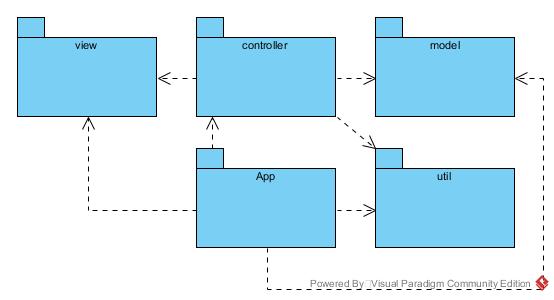
\includegraphics[scale=4, max width=\textwidth, max height=\myheight]{../img/diagrammiClassi/architetturaClient.png}
		\caption{Diagramma package - client}
	\end{figure}
\end{center}

Al fine di rendere il diagramma delle classi del client più leggibile si è deciso di dividerlo, quindi di seguito si può vedere il diagramma delle classi, con le relative relazione, di \texttt{view}, \texttt{controller} e \texttt{util}.
\begin{center}
	\begin{figure}[H]
		\centering 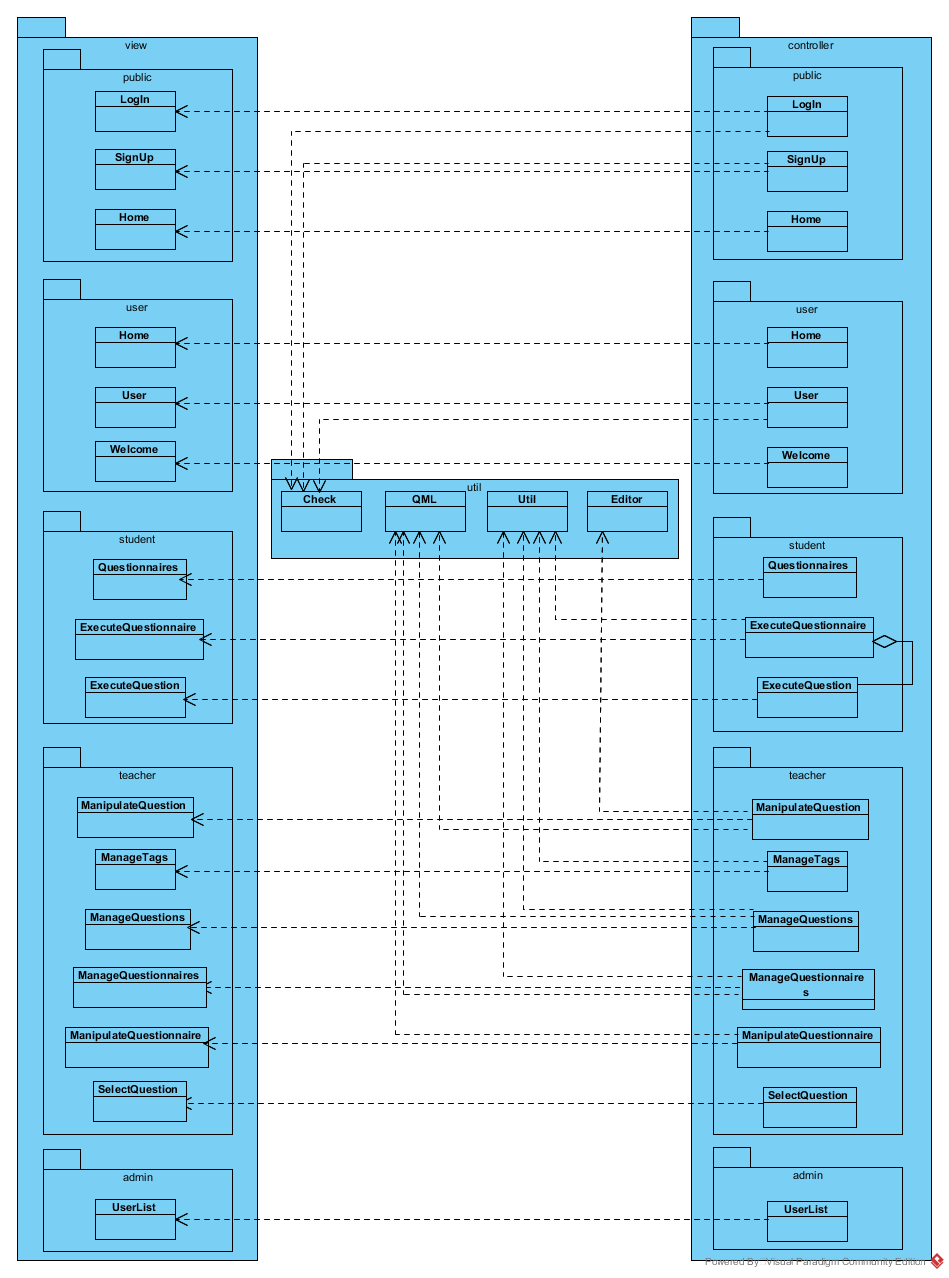
\includegraphics[scale=4, max width=\textwidth, max height=\myheight]{../img/diagrammiClassi/client/viewControllerUtil.png}
		\caption{Diagramma package - client::view, client::controller, client::util}
	\end{figure}
\end{center}

Seguendo si può vedere il diagramma delle classi di \texttt{controller}, \texttt{model} e \texttt{app}.
\begin{center}
	\begin{figure}[H]
		\centering 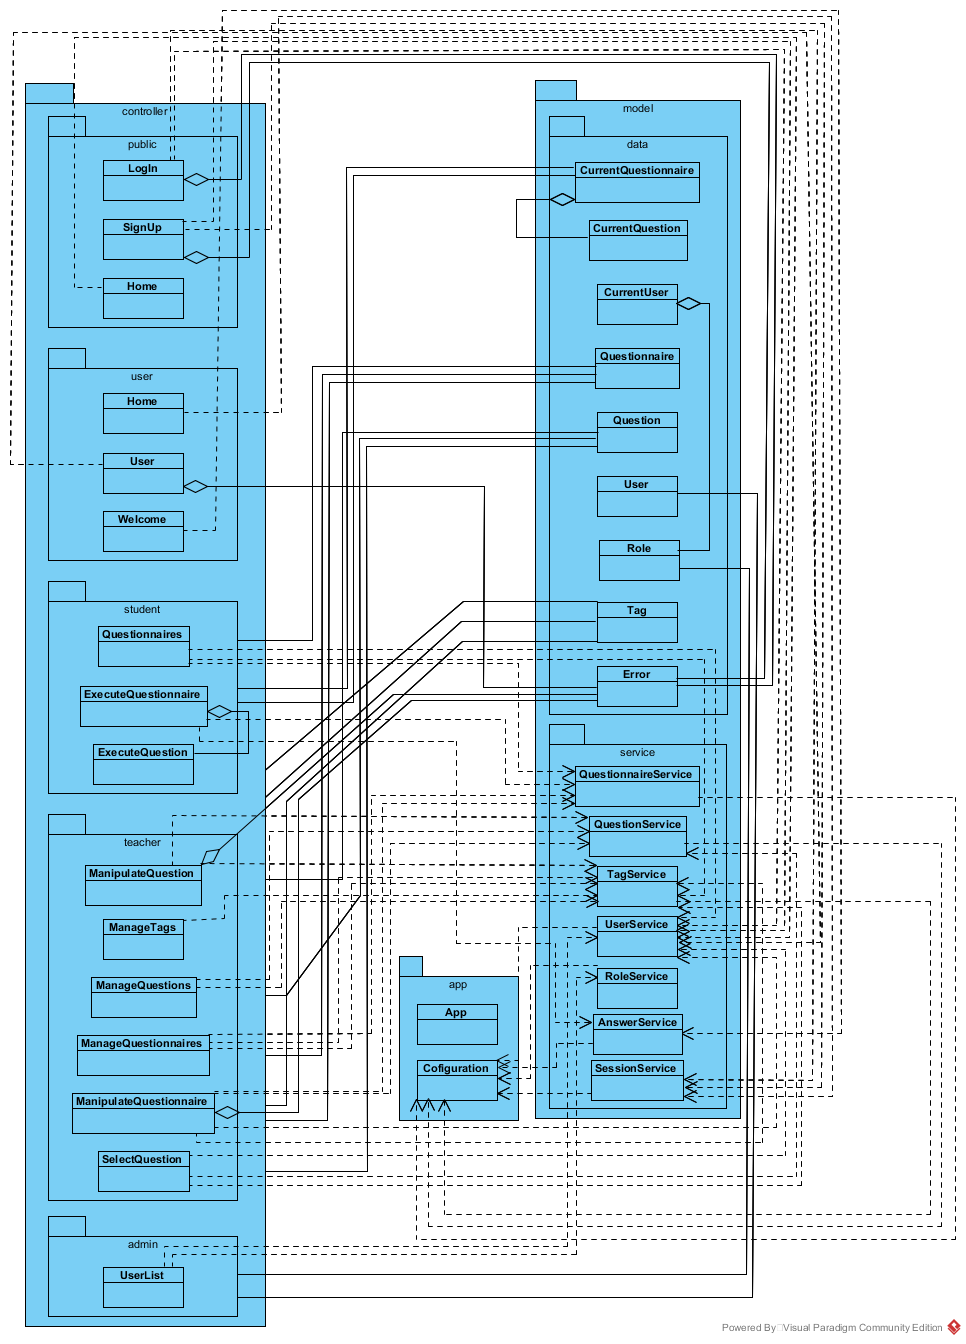
\includegraphics[scale=4, max width=\textwidth, max height=\myheight]{../img/diagrammiClassi/client/controllerModelApp.png}
		\caption{Diagramma package - client::controller, client::model, client::app}
	\end{figure}
\end{center}

\subsection{Introduzione alle classi view}
Le classi \mgls{view}, che hanno una corrispondenza uno ad uno con le classi \mgls{controller} (logica applicativa), sono scritte come pagine \mgls{html}, quindi sono sprovviste di campi dati o metodi.
Per permette l’interazione delle le \mgls{view} \mgls{html} con l'applicazione, vengono usate le direttive di \mgls{angularjs} le quali permettono, attraverso l'utilizzo del pattern MVVM e in particolare del pattern observer,
di notificare ai \mgls{controller} gli eventi innescati dall'utente attraverso l'User Interface. 
Inoltre grazie al two-way data binding di \mgls{angularjs} le viste e i dati sono sincronizzati e qualsiasi modifica ad uno di questi componenti verrà rispecchiata automaticamente sull'altro. 
Al fine di rendere maggiormente comprensibile la descrizione testuale delle classi del \mgls{package} \mgls{view}, verranno elencate le direttive \mgls{angularjs} usate dalle stesse per rendere le pagine \mgls{html} dinamiche:

\begin{itemize}
	\item \textbf{ng-controller:} permette l’attivazione del \mgls{controller} dedicato al corrispondente template \mgls{html}
	\item \textbf{ng-model:} permette di creare un legame tra le variabili presenti nel \$scope e i campi di tipo input della pagina \mgls{html}
	\item \textbf{ng-click:} Rileva una scelta dell’utente e attiva una funzione definita nel \mgls{controller} associato
	\item \textbf{ng-show:} Permette di visualizzare o meno del contenuti \mgls{html} a seconda se una determina condizione sia verificata
	\item \textbf{ng-change:} Permette di rilevare un cambiamento su un determinato elemento di una form
	\item \textbf{ng-repeat:} Permette di iterare ogni elemento di una lista e di poterlo utilizzare all’interno del template \mgls{html} grazie alla direttiva ng-bind potendone ricavare dati o eseguire metodi su di esso
	\item \textbf{ng-submit:} Rileva una scelta di invio dati dell’utente e attiva una funzione
	\item \textbf{ng-class:} Permette di associare una determinata classe, a un elemento del template, qualora la condizione specificata risultasse vera
	\item \textbf{ng-blur:} Permette di impostare delle azioni quando un elemento \mgls{html} perde il focus
	\item \textbf{ng-bind:} Permette di rimpiazzare il contenuto di un elemento con il valore dato dall’espressione definita. Questa direttiva viene preferita all’uso dell’operatore {{ }}. Viene utilizzata per stampare il valore degli elementi che si stanno iterando tramite la direttiva ng-repeat
	\item \textbf{ng-bind-html:} Permette di rimpiazzare il contenuto di un elemento con del codice \mgls{html} che non viene interpretato come stringa ma come codice della pagina. Viene usato per il valore dato dall’espressione definita. Questa direttiva viene preferita all’uso dell’operatore {{ }}
	\item \textbf{ng-include:} Permette recupera, compila e include un frammento \mgls{html} esterno
	\item \textbf{ng-disable:} Permette di impostare l'attributo disabled su un determinato elemento, il che permette di renderlo non editabile dall'utente
	\item \textbf{ng-switch:} E' usata per scambiare la struttura del'\mgls{dom} sul template \mgls{html} in base ad un espressione dello scope. Funziona in maniera analoga ad ng-include tuttavia ,invece di scraicare il codice del teamplate \mgls{html} da includere, ngSwitch sceglie uno degli elementi al suo interno (appoggiandosi alle direttive ng-switch-default e ng-switch-when) e lo rende visibile basandosi sul valore ottenuto dall'espressione valutata
	\item \textbf{ng-true-value:} Permette l'esecuzione di funzioni javascript se il valore ottenuto dall'espressione valutata è true
	\item \textbf{ng-false-value:} Permette l'esecuzione di funzioni javascript se il valore ottenuto dall'espressione valutata è false
	\end{itemize}

\subsection{client::view}
È il package che contiene tutte le classi che costituiscono la view del client. 
Ogni componente si occupa della visualizzazione di una particolare porzione dell'interfaccia di un utente.

\begin{center}
	\begin{figure}[H]
		\centering 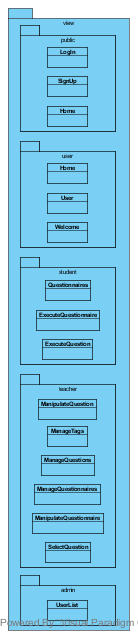
\includegraphics[scale=4, max width=\textwidth, max height=\myheight]{../img/diagrammiClassi/client/view.png}
		\caption{Diagramma package - client::view}
	\end{figure}
\end{center}\subsubsection{client::view::public}
È il package che contiene tutte le classi che costituiscono la view della porzione publica di client. Ogni componente si occupa della visualizzazione di una particolare porzione dell'interfaccia di un utente non autenticato.\begin{center}
	\begin{figure}[H]
		\centering 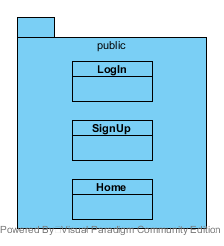
\includegraphics[scale=4, max width=\textwidth, max height=\myheight]{../img/diagrammiClassi/client/view/public.png}
		\caption{Diagramma package - client::view::public}
	\end{figure}
\end{center}\hypertarget{client::view::public::LogIn}{}
\subsubsubsection[LogIn]{client::view::public::LogIn}
\begin{description}
\item[Descrizione] \hfill \\
La classe rappresenta un template HTML che si occupa della visualizzazione dell'area di autenticazione
\end{description}

\vspace{0.5cm}
\hypertarget{client::view::public::SignUp}{}
\subsubsubsection[SignUp]{client::view::public::SignUp}
\begin{description}
\item[Descrizione] \hfill \\
La classe rappresenta un template HTML che si occupa della visualizzazione sul client dell'area di registrazione
\end{description}

\vspace{0.5cm}
\hypertarget{client::view::public::Home}{}
\subsubsubsection[Home]{client::view::public::Home}
\begin{description}
\item[Descrizione] \hfill \\
La classe rappresenta un template HTML che si occupa della visualizzazione della home page di un'utente generico. Questa permetterà di svolgere questionari anche senza autenticazione.
\end{description}

\vspace{0.5cm}
\subsubsection{client::view::student}
È il package che contiene tutte le classi che costituiscono la view della porzione di client per uno studente. Ogni componente si occupa della visualizzazione di una particolare porzione dell'interfaccia di uno studente.\begin{center}
	\begin{figure}[H]
		\centering 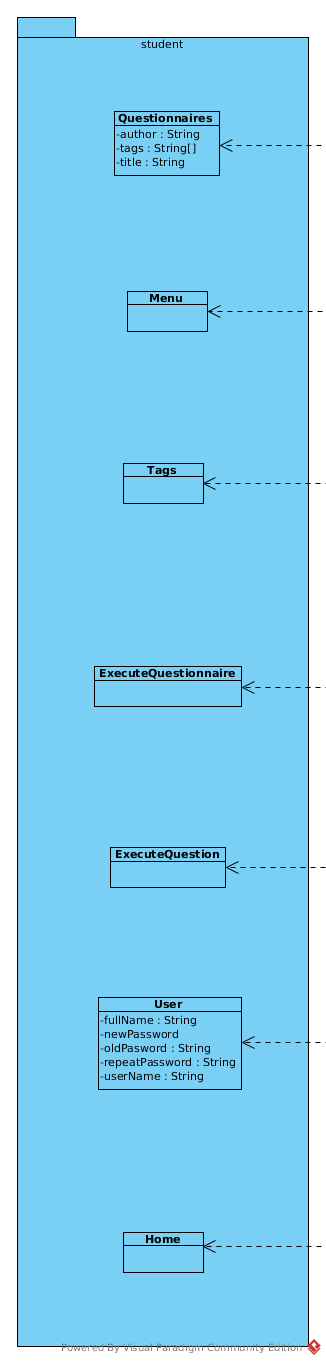
\includegraphics[scale=4, max width=\textwidth, max height=\myheight]{../img/diagrammiClassi/client/view/student.png}
		\caption{Diagramma package - client::view::student}
	\end{figure}
\end{center}\hypertarget{client::view::student::Questionnaires}{}
\subsubsubsection[Questionnaires]{client::view::student::Questionnaires}
\begin{description}
\item[Descrizione] \hfill \\
La classe rappresenta un template HTML che si occupa della visualizzazione della lista dei questionari eseguibili
\end{description}

\vspace{0.5cm}
\hypertarget{client::view::student::ExecuteQuestionnaire}{}
\subsubsubsection[ExecuteQuestionnaire]{client::view::student::ExecuteQuestionnaire}
\begin{description}
\item[Descrizione] \hfill \\
La classe rappresenta un template HTML che si occupa della visualizzazione di un questionario in esecuzione
\end{description}

\vspace{0.5cm}
\hypertarget{client::view::student::ExecuteQuestion}{}
\subsubsubsection[ExecuteQuestion]{client::view::student::ExecuteQuestion}
\begin{description}
\item[Descrizione] \hfill \\
La classe rappresenta un template HTML che si occupa della visualizzazione una domanda in esecuzione
\end{description}

\vspace{0.5cm}
\subsubsection{client::view::teacher}
È il package che contiene tutte le classi che costituiscono la view della porzione di client per un docente. Ogni componente si occupa della visualizzazione di una particolare porzione dell'interfaccia di un docente.\begin{center}
	\begin{figure}[H]
		\centering 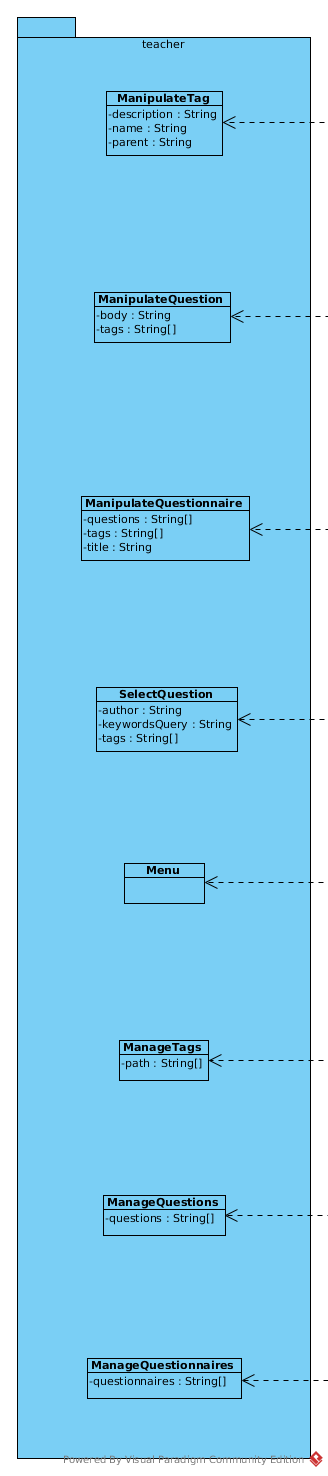
\includegraphics[scale=4, max width=\textwidth, max height=\myheight]{../img/diagrammiClassi/client/view/teacher.png}
		\caption{Diagramma package - client::view::teacher}
	\end{figure}
\end{center}\hypertarget{client::view::teacher::ManipulateQuestion}{}
\subsubsubsection[ManipulateQuestion]{client::view::teacher::ManipulateQuestion}
\begin{description}
\item[Descrizione] \hfill \\
La classe rappresenta un template HTML che si occupa delle visualizzazione della gestione della domanda
\end{description}

\vspace{0.5cm}
\hypertarget{client::view::teacher::ManipulateQuestionnaire}{}
\subsubsubsection[ManipulateQuestionnaire]{client::view::teacher::ManipulateQuestionnaire}
\begin{description}
\item[Descrizione] \hfill \\
La classe rappresenta un template HTML che si occupa della visualizzazione della gestione del questionario 
\end{description}

\vspace{0.5cm}
\hypertarget{client::view::teacher::SelectQuestion}{}
\subsubsubsection[SelectQuestion]{client::view::teacher::SelectQuestion}
\begin{description}
\item[Descrizione] \hfill \\
La classe rappresenta un template HTML che si occupa della visualizzazione di selezione delle domande
\end{description}

\vspace{0.5cm}
\hypertarget{client::view::teacher::ManageTags}{}
\subsubsubsection[ManageTags]{client::view::teacher::ManageTags}
\begin{description}
\item[Descrizione] \hfill \\
La classe rappresenta un template HTML che si occupa della visualizzazione degli argomenti per selezionare un eventuale argomento da gestire
\end{description}

\vspace{0.5cm}
\hypertarget{client::view::teacher::ManageQuestions}{}
\subsubsubsection[ManageQuestions]{client::view::teacher::ManageQuestions}
\begin{description}
\item[Descrizione] \hfill \\
La classe rappresenta un template HTML che si occupa della visualizzazione della lista delle proprie domande per selezionare la domanda da gestire
\end{description}

\vspace{0.5cm}
\hypertarget{client::view::teacher::ManageQuestionnaires}{}
\subsubsubsection[ManageQuestionnaires]{client::view::teacher::ManageQuestionnaires}
\begin{description}
\item[Descrizione] \hfill \\
La classe rappresenta un template HTML che si occupa della visualizzazione della lista dei propri questionari per selezionare il questionario da gestire
\end{description}

\vspace{0.5cm}
\subsubsection{client::view::admin}
È il package che contiene tutte le classi che costituiscono la view della porzione di client per un amministratore. Ogni componente si occupa della visualizzazione di una particolare porzione dell'interfaccia di un amministratore.\begin{center}
	\begin{figure}[H]
		\centering 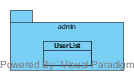
\includegraphics[scale=4, max width=\textwidth, max height=\myheight]{../img/diagrammiClassi/client/view/admin.png}
		\caption{Diagramma package - client::view::admin}
	\end{figure}
\end{center}\hypertarget{client::view::admin::UsersList}{}
\subsubsubsection[UsersList]{client::view::admin::UsersList}
\begin{description}
\item[Descrizione] \hfill \\
La classe rappresenta un template HTML che si occupa della visualizzazione della lista degli utenti.Consente di applicare un filtro ai risultari tra FullName, Role, UserName per la selezione di un utente per la gestione delle sue informazioni.
\end{description}

\vspace{0.5cm}
\subsubsection{client::view::user}
È il package che contiene tutte le classi che costituiscono la view della porzione di client per un'utente generico registrato. Ogni componente si occupa della visualizzazione di una particolare porzione dell'interfaccia di un'utente generico registrato.\begin{center}
	\begin{figure}[H]
		\centering 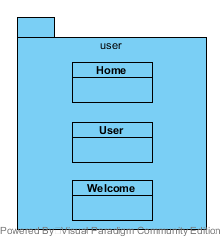
\includegraphics[scale=4, max width=\textwidth, max height=\myheight]{../img/diagrammiClassi/client/view/user.png}
		\caption{Diagramma package - client::view::user}
	\end{figure}
\end{center}\hypertarget{client::view::user::Welcome}{}
\subsubsubsection[Welcome]{client::view::user::Welcome}
\begin{description}
\item[Descrizione] \hfill \\
La classe rappresenta un template HTML che si occupa della visualizzazione della pagina di benvenuto
\end{description}

\vspace{0.5cm}
\hypertarget{client::view::user::Home}{}
\subsubsubsection[Home]{client::view::user::Home}
\begin{description}
\item[Descrizione] \hfill \\
La classe rappresenta un template HTML che si occupa della visualizzazione della home page di un'utente generico autenticato
\end{description}

\vspace{0.5cm}
\hypertarget{client::view::user::User}{}
\subsubsubsection[User]{client::view::user::User}
\begin{description}
\item[Descrizione] \hfill \\
la classe rappresenta un template HTML che si occupa di visualizzare la pagina per la gestione del profilo di un'utente generico registrato
\end{description}

\vspace{0.5cm}
\subsection{client::model}
E' il package che contiene le classi dei modelli di dati utilizzati
dal client e i servizi che mettono in comunicazione esso con il server
attraverso i diversi servizi REST.\begin{center}
	\begin{figure}[H]
		\centering 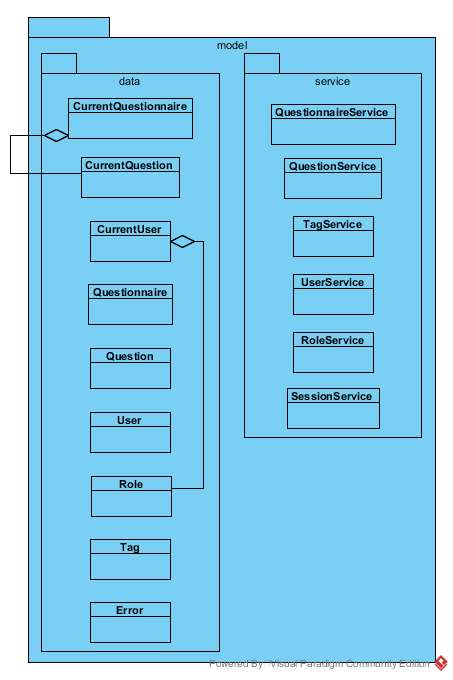
\includegraphics[scale=4, max width=\textwidth, max height=\myheight]{../img/diagrammiClassi/client/model.png}
		\caption{Diagramma package - client::model}
	\end{figure}
\end{center}\subsubsection{client::model::data}
Questo package si occupa della modellazione dei dati utili al client.\begin{center}
	\begin{figure}[H]
		\centering 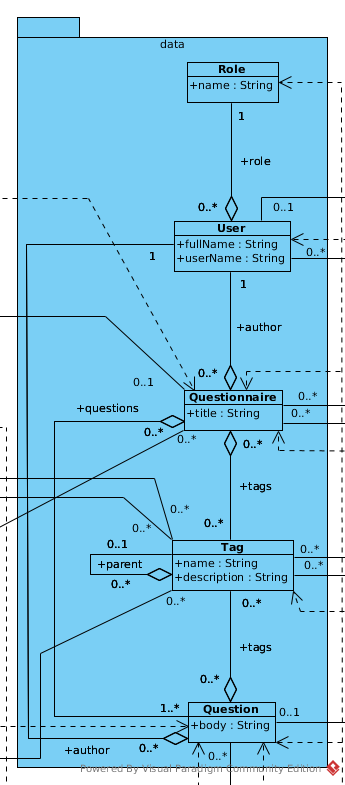
\includegraphics[scale=4, max width=\textwidth, max height=\myheight]{../img/diagrammiClassi/client/model/data.png}
		\caption{Diagramma package - client::model::data}
	\end{figure}
\end{center}\hypertarget{client::model::data::Questionnaire}{}
\subsubsubsection[Questionnaire]{client::model::data::Questionnaire}
\begin{figure}[H]
	\centering
	\begin{tikzpicture}
	\umlclass{client::model::data::Questionnaire} {--questions : String[]\\--tags : String[]\\--author : String\\--title : String\\--id : String}{+Questionnaire(author : String, id : String, questions : String[], tags : String[], title : String)\\+getQuestions() : String[]\\+getTags() : String[]\\+getAuthor() : String\\+getTitle() : String\\+getId() : String\\+setQuestions(questions : String[]) : void\\+setTags(tags : String[]) : void\\+setAuthor(author : String) : void\\+setTitle(title : String) : void\\+setId(id : String) : void}
	\end{tikzpicture}
	\caption{Diagramma classe - client::model::data::Questionnaire}
\end{figure}\begin{description}
\item[Descrizione] \hfill \\
Questa classe modella il tipo di dato "questionario" nella rappresentazione locale dei dati lato client
\item[Relazioni con altre classi] \hfill \\
\vspace{-7mm}
\begin{description}
	\item[\hyperlink{client::controller::teacher::ManipulateQuestionnaire}{client::controller::teacher::ManipulateQuestionnaire}] \hfill \\
	Relazione entrante, oggetto che rappresenta un questionario
	\item[\hyperlink{client::controller::student::Questionnaires}{client::controller::student::Questionnaires}] \hfill \\
	Relazione entrante, lista di questionari
	\item[\hyperlink{client::controller::teacher::ManageQuestionnaires}{client::controller::teacher::ManageQuestionnaires}] \hfill \\
	Relazione entrante, questionari visualizzati nella view
\end{description}

\item[Attributi] \hfill \\
\vspace{-7mm}
\begin{itemize}
	\item questions : String[] $\rightarrow$ insieme di ID di riferimenti a Question
	\item tags : String[] $\rightarrow$ lista di ID di riferimenti ad argomenti 
	\item author : String $\rightarrow$ ID dell'autore del questionario
	\item title : String $\rightarrow$ nome del questionario
	\item id : String $\rightarrow$ ID del Questionnaire
\end{itemize}

\item[Metodi] \hfill \\
\vspace{-7mm}
\begin{itemize}
	\item Questionnaire(author : String, id : String, questions : String[], tags : String[], title : String) $\rightarrow$ costruttore della classe\begin{itemize}
		\item author $\rightarrow$ ID dell'autore del questionario
		\item id $\rightarrow$ ID del Questionnaire
		\item questions $\rightarrow$ insieme di ID di riferimenti a Question
		\item tags $\rightarrow$ lista di ID di riferimenti ad argomenti
		\item title $\rightarrow$ nome del questionario
	\end{itemize}
	
	\item getQuestions() : String[] $\rightarrow$ metodo che restituisce il valore del campo dati questions
	\item getTags() : String[] $\rightarrow$ metodo che restituisce il valore del campo dati tags
	\item getAuthor() : String $\rightarrow$ metodo che restituisce il valore del campo dati author
	\item getTitle() : String $\rightarrow$ metodo che restituisce il valore del campo dati title
	\item getId() : String $\rightarrow$ metodo che restituisce il valore del campo dati id
	\item setQuestions(questions : String[]) : void $\rightarrow$ metodo che cambia il valore del campo dati questions\begin{itemize}
		\item questions $\rightarrow$ insieme di ID di riferimenti a Question
	\end{itemize}
	
	\item setTags(tags : String[]) : void $\rightarrow$ metodo che cambia il valore del campo dati tags\begin{itemize}
		\item tags $\rightarrow$ lista di ID di riferimenti ad argomenti 
	\end{itemize}
	
	\item setAuthor(author : String) : void $\rightarrow$ metodo che cambia il valore del campo dati author\begin{itemize}
		\item author $\rightarrow$ ID dell'autore del questionario
	\end{itemize}
	
	\item setTitle(title : String) : void $\rightarrow$ metodo che cambia il valore del campo dati title\begin{itemize}
		\item title $\rightarrow$ nome del questionario
	\end{itemize}
	
	\item setId(id : String) : void $\rightarrow$ metodo che cambia il valore del campo dati id\begin{itemize}
		\item id $\rightarrow$ ID del Questionnaire
	\end{itemize}
	
\end{itemize}

\end{description}

\vspace{0.5cm}
\hypertarget{client::model::data::Question}{}
\subsubsubsection[Question]{client::model::data::Question}
\begin{figure}[H]
	\centering
	\begin{tikzpicture}
	\umlclass{client::model::data::Question} {--body : String\\--author : String\\--tags  : String[]\\--id : String}{+Question(author : String, body : String, id : String, tags : String[])\\+getBody() : String\\+getAuthor() : String\\+getTags () : String[]\\+getId() : String\\+setBody(body : String) : void\\+setAuthor(author : String) : void\\+setTags (tags  : String[]) : void\\+setId(id : String) : void}
	\end{tikzpicture}
	\caption{Diagramma classe - client::model::data::Question}
\end{figure}\begin{description}
\item[Descrizione] \hfill \\
Questa classe modella il tipo di dato "domanda" nella rappresentazione locale dei dati lato client
\item[Relazioni con altre classi] \hfill \\
\vspace{-7mm}
\begin{description}
	\item[\hyperlink{client::controller::teacher::ManipulateQuestion}{client::controller::teacher::ManipulateQuestion}] \hfill \\
	Relazione entrante, oggetto che rappresenta una singola domanda
	\item[\hyperlink{client::controller::teacher::ManageQuestions}{client::controller::teacher::ManageQuestions}] \hfill \\
	Relazione entrante, domande visualizzate nella view
	\item[\hyperlink{client::controller::teacher::SelectQuestion}{client::controller::teacher::SelectQuestion}] \hfill \\
	Relazione entrante, domande visualizzate nella view
\end{description}

\item[Attributi] \hfill \\
\vspace{-7mm}
\begin{itemize}
	\item body : String $\rightarrow$ e' la rappresentazione testuale della domanda
	\item author : String $\rightarrow$ ID dell'autore della domanda
	\item tags  : String[] $\rightarrow$ lista di ID di riferimenti ad argomenti
	\item id : String $\rightarrow$ ID della Question
\end{itemize}

\item[Metodi] \hfill \\
\vspace{-7mm}
\begin{itemize}
	\item Question(author : String, body : String, id : String, tags : String[]) $\rightarrow$ costruttore della classe\begin{itemize}
		\item author $\rightarrow$ ID dell'autore della domanda
		\item body $\rightarrow$ e' la rappresentazione testuale della domanda
		\item id $\rightarrow$ ID della Question
		\item tags $\rightarrow$ lista di ID di riferimenti ad argomenti
	\end{itemize}
	
	\item getBody() : String $\rightarrow$ metodo che restituisce il valore del campo dati body
	\item getAuthor() : String $\rightarrow$ metodo che restituisce il valore del campo dati author
	\item getTags () : String[] $\rightarrow$ metodo che restituisce il valore del campo dati tags 
	\item getId() : String $\rightarrow$ metodo che restituisce il valore del campo dati id
	\item setBody(body : String) : void $\rightarrow$ metodo che cambia il valore del campo dati body\begin{itemize}
		\item body $\rightarrow$ e' la rappresentazione testuale della domanda
	\end{itemize}
	
	\item setAuthor(author : String) : void $\rightarrow$ metodo che cambia il valore del campo dati author\begin{itemize}
		\item author $\rightarrow$ ID dell'autore della domanda
	\end{itemize}
	
	\item setTags (tags  : String[]) : void $\rightarrow$ metodo che cambia il valore del campo dati tags \begin{itemize}
		\item tags  $\rightarrow$ lista di ID di riferimenti ad argomenti
	\end{itemize}
	
	\item setId(id : String) : void $\rightarrow$ metodo che cambia il valore del campo dati id\begin{itemize}
		\item id $\rightarrow$ ID della Question
	\end{itemize}
	
\end{itemize}

\end{description}

\vspace{0.5cm}
\hypertarget{client::model::data::Tag}{}
\subsubsubsection[Tag]{client::model::data::Tag}
\begin{figure}[H]
	\centering
	\begin{tikzpicture}
	\umlclass{client::model::data::Tag} {--name : String\\--description : String\\--id : String}{+Tag(description : String, id : String, name : String)\\+getName() : String\\+getDescription() : String\\+getId() : String\\+setName(name : String) : void\\+setDescription(description : String) : void\\+setId(id : String) : void}
	\end{tikzpicture}
	\caption{Diagramma classe - client::model::data::Tag}
\end{figure}\begin{description}
\item[Descrizione] \hfill \\
Questa classe modella il tag argomento di un questionario e/o di una domanda nella rappresentazione locale dei dati lato client
\item[Relazioni con altre classi] \hfill \\
\vspace{-7mm}
\begin{description}
	\item[\hyperlink{client::controller::teacher::ManageTags}{client::controller::teacher::ManageTags}] \hfill \\
	Relazione entrante, tags visualizzati nella view
	\item[\hyperlink{client::controller::teacher::ManipulateQuestion}{client::controller::teacher::ManipulateQuestion}] \hfill \\
	Relazione entrante, argomenti che compaiono nei suggerimenti
	\item[\hyperlink{client::controller::teacher::ManipulateQuestionnaire}{client::controller::teacher::ManipulateQuestionnaire}] \hfill \\
	Relazione entrante, argomenti che compaiono nei suggerimenti
\end{description}

\item[Attributi] \hfill \\
\vspace{-7mm}
\begin{itemize}
	\item name : String $\rightarrow$ nome dell'argomento
	\item description : String $\rightarrow$ descrizione dell'argomento
	\item id : String $\rightarrow$ ID del Tag
\end{itemize}

\item[Metodi] \hfill \\
\vspace{-7mm}
\begin{itemize}
	\item Tag(description : String, id : String, name : String) $\rightarrow$ costruttore della classe\begin{itemize}
		\item description $\rightarrow$ descrizione dell'argomento
		\item id $\rightarrow$ ID del Tag
		\item name $\rightarrow$ nome dell'argomento
	\end{itemize}
	
	\item getName() : String $\rightarrow$ metodo che restituisce il valore del campo dati name
	\item getDescription() : String $\rightarrow$ metodo che restituisce il valore del campo dati description
	\item getId() : String $\rightarrow$ metodo che restituisce il valore del campo dati id
	\item setName(name : String) : void $\rightarrow$ metodo che cambia il valore del campo dati name\begin{itemize}
		\item name $\rightarrow$ nome dell'argomento
	\end{itemize}
	
	\item setDescription(description : String) : void $\rightarrow$ metodo che cambia il valore del campo dati description\begin{itemize}
		\item description $\rightarrow$ descrizione dell'argomento
	\end{itemize}
	
	\item setId(id : String) : void $\rightarrow$ metodo che cambia il valore del campo dati id\begin{itemize}
		\item id $\rightarrow$ ID del Tag
	\end{itemize}
	
\end{itemize}

\end{description}

\vspace{0.5cm}
\hypertarget{client::model::data::Role}{}
\subsubsubsection[Role]{client::model::data::Role}
\begin{figure}[H]
	\centering
	\begin{tikzpicture}
	\umlclass{client::model::data::Role} {--name : String\\--id : String}{+Role(id : String, name : String)\\+getName() : String\\+getId() : String\\+setName(name : String) : void\\+setId(id : String) : void}
	\end{tikzpicture}
	\caption{Diagramma classe - client::model::data::Role}
\end{figure}\begin{description}
\item[Descrizione] \hfill \\
Questa classe modella il ruolo e i permessi di un utente autenticato nel sistema
\item[Relazioni con altre classi] \hfill \\
\vspace{-7mm}
\begin{description}
	\item[\hyperlink{client::controller::admin::UsersList}{client::controller::admin::UsersList}] \hfill \\
	Relazione entrante, lista di tutti i ruoli che può assumere un utente
	\item[\hyperlink{client::model::data::CurrentUser}{client::model::data::CurrentUser}] \hfill \\
	Relazione entrante, role del ruolo dell'utente
\end{description}

\item[Attributi] \hfill \\
\vspace{-7mm}
\begin{itemize}
	\item name : String $\rightarrow$ e' il ruolo che un utente può assumere
	\item id : String $\rightarrow$ ID del Role
\end{itemize}

\item[Metodi] \hfill \\
\vspace{-7mm}
\begin{itemize}
	\item Role(id : String, name : String) $\rightarrow$ costruttore della classe\begin{itemize}
		\item id $\rightarrow$ ID del Role
		\item name $\rightarrow$ e' il ruolo che un utente può assumere
	\end{itemize}
	
	\item getName() : String $\rightarrow$ metodo che restituisce il valore del campo dati name
	\item getId() : String $\rightarrow$ metodo che restituisce il valore del campo dati id
	\item setName(name : String) : void $\rightarrow$ metodo che cambia il valore del campo dati name\begin{itemize}
		\item name $\rightarrow$ e' il ruolo che un utente può assumere
	\end{itemize}
	
	\item setId(id : String) : void $\rightarrow$ metodo che cambia il valore del campo dati id\begin{itemize}
		\item id $\rightarrow$ ID del Role
	\end{itemize}
	
\end{itemize}

\end{description}

\vspace{0.5cm}
\hypertarget{client::model::data::User}{}
\subsubsubsection[User]{client::model::data::User}
\begin{figure}[H]
	\centering
	\begin{tikzpicture}
	\umlclass{client::model::data::User} {--role : String\\--fullName : String\\--userName : String\\--id : String}{+User(fullName : String, id : String, role : String, userName : String)\\+getRole() : String\\+getFullName() : String\\+getUserName() : String\\+getId() : String\\+setRole(role : String) : void\\+setFullName(fullName : String) : void\\+setUserName(userName : String) : void\\+setId(id : String) : void}
	\end{tikzpicture}
	\caption{Diagramma classe - client::model::data::User}
\end{figure}\begin{description}
\item[Descrizione] \hfill \\
Questa classe modella le informazioni del profilo di un utente autenticato nel sistema
\item[Relazioni con altre classi] \hfill \\
\vspace{-7mm}
\begin{description}
	\item[\hyperlink{client::controller::admin::UsersList}{client::controller::admin::UsersList}] \hfill \\
	Relazione entrante, lista di utenti
\end{description}

\item[Attributi] \hfill \\
\vspace{-7mm}
\begin{itemize}
	\item role : String $\rightarrow$ ID del Role del ruolo dell'utente
	\item fullName : String $\rightarrow$ nome completo dell'utente
	\item userName : String $\rightarrow$ userName dell'utente
	\item id : String $\rightarrow$ ID dell'User
\end{itemize}

\item[Metodi] \hfill \\
\vspace{-7mm}
\begin{itemize}
	\item User(fullName : String, id : String, role : String, userName : String) $\rightarrow$ costruttore della classe\begin{itemize}
		\item fullName $\rightarrow$ nome completo dell'utente
		\item id $\rightarrow$ ID dell'User
		\item role $\rightarrow$ ID del Role del ruolo dell'utente
		\item userName $\rightarrow$ userName dell'utente
	\end{itemize}
	
	\item getRole() : String $\rightarrow$ metodo che restituisce il valore del campo dati role
	\item getFullName() : String $\rightarrow$ metodo che restituisce il valore del campo dati fullName
	\item getUserName() : String $\rightarrow$ metodo che restituisce il valore del campo dati userName
	\item getId() : String $\rightarrow$ metodo che restituisce il valore del campo dati id
	\item setRole(role : String) : void $\rightarrow$ metodo che cambia il valore del campo dati role\begin{itemize}
		\item role $\rightarrow$ ID del Role del ruolo dell'utente
	\end{itemize}
	
	\item setFullName(fullName : String) : void $\rightarrow$ metodo che cambia il valore del campo dati fullName\begin{itemize}
		\item fullName $\rightarrow$ nome completo dell'utente
	\end{itemize}
	
	\item setUserName(userName : String) : void $\rightarrow$ metodo che cambia il valore del campo dati userName\begin{itemize}
		\item userName $\rightarrow$ userName dell'utente
	\end{itemize}
	
	\item setId(id : String) : void $\rightarrow$ metodo che cambia il valore del campo dati id\begin{itemize}
		\item id $\rightarrow$ ID dell'User
	\end{itemize}
	
\end{itemize}

\end{description}

\vspace{0.5cm}
\hypertarget{client::model::data::CurrentQuestion}{}
\subsubsubsection[CurrentQuestion]{client::model::data::CurrentQuestion}
\begin{figure}[H]
	\centering
	\begin{tikzpicture}
	\umlclass{client::model::data::CurrentQuestion} {--body : String\\--answer : String\\--type : String\\--answers : String []\\--selectedAnswer : String}{+CurrentQuestion(question : Question)\\+point() : Json\\+getBody() : String\\+getAnswer() : String\\+getType() : String\\+setBody(body : String) : void\\+setAnswer(answer : String) : void\\+setType(type : String) : void\\+getAnswers() : String []\\+getSelectedAnswer() : String\\+setAnswers(answers : String []) : void\\+setSelectedAnswer(selectedAnswer : String) : void}
	\end{tikzpicture}
	\caption{Diagramma classe - client::model::data::CurrentQuestion}
\end{figure}\begin{description}
\item[Descrizione] \hfill \\
La classe che modella la domanda in esecuzione
\item[Relazioni con altre classi] \hfill \\
\vspace{-7mm}
\begin{description}
	\item[\hyperlink{client::model::data::CurrentQuestionnaire}{client::model::data::CurrentQuestionnaire}] \hfill \\
	Relazione entrante, lista di domande del questionario corrente
\end{description}

\item[Attributi] \hfill \\
\vspace{-7mm}
\begin{itemize}
	\item body : String $\rightarrow$ contiene il corpo della domanda corrente 
	\item answer : String $\rightarrow$ contiene la risposta alla domanda corrente
	\item type : String $\rightarrow$ oggetto che rappresenta la tipologia della domanda
	\item answers : String [] $\rightarrow$ oggetto che rappresenta una lista di risposte
	\item selectedAnswer : String $\rightarrow$ oggetto che rappresenta la risposta selezionata
\end{itemize}

\item[Metodi] \hfill \\
\vspace{-7mm}
\begin{itemize}
	\item CurrentQuestion(question : Question) $\rightarrow$ costruttore della classe\begin{itemize}
		\item question $\rightarrow$ contiene il riferimento all'oggetto Question associato
	\end{itemize}
	
	\item point() : Json $\rightarrow$ restituisce i punti relativi alla domanda risposta
	
	Metodo che restituisce un oggetto di tipo json con attributi 'point' e 'tot' che contengono due interi rappresentanti i punti totalizzati sui punti totali del risposta
	\item getBody() : String $\rightarrow$ metodo che restituisce il valore del campo dati body
	\item getAnswer() : String $\rightarrow$ metodo che restituisce il valore del campo dati answer
	\item getType() : String $\rightarrow$ metodo che restituisce il valore del campo dati type
	\item setBody(body : String) : void $\rightarrow$ metodo che cambia il valore del campo dati body\begin{itemize}
		\item body $\rightarrow$ contiene il corpo della domanda corrente 
	\end{itemize}
	
	\item setAnswer(answer : String) : void $\rightarrow$ metodo che cambia il valore del campo dati answer\begin{itemize}
		\item answer $\rightarrow$ contiene la risposta alla domanda corrente
	\end{itemize}
	
	\item setType(type : String) : void $\rightarrow$ metodo che cambia il valore del campo dati type\begin{itemize}
		\item type $\rightarrow$ oggetto che rappresenta la tipologia della domanda
	\end{itemize}
	
	\item getAnswers() : String [] $\rightarrow$ metodo che restituisce il valore del campo dati answers
	\item getSelectedAnswer() : String $\rightarrow$ metodo che restituisce il valore del campo dati selectedAnswer
	\item setAnswers(answers : String []) : void $\rightarrow$ metodo che cambia il valore del campo dati answers\begin{itemize}
		\item answers $\rightarrow$ oggetto che rappresenta una lista di risposte
	\end{itemize}
	
	\item setSelectedAnswer(selectedAnswer : String) : void $\rightarrow$ metodo che cambia il valore del campo dati selectedAnswer\begin{itemize}
		\item selectedAnswer $\rightarrow$ oggetto che rappresenta la risposta selezionata
	\end{itemize}
	
\end{itemize}

\end{description}

\vspace{0.5cm}
\hypertarget{client::model::data::CurrentQuestionnaire}{}
\subsubsubsection[CurrentQuestionnaire]{client::model::data::CurrentQuestionnaire}
\begin{figure}[H]
	\centering
	\begin{tikzpicture}
	\umlclass{client::model::data::CurrentQuestionnaire} {--tags : String[]\\--currentNumber : int\\--questionNumber : int\\--questions : CurrentQuestion[]\\--title : String}{+getNext () : CurrentQuestion\\+getPrevious() : CurrentQuestion\\+checkAnswers() : boolean\\+CurrentQuestionnaire(questions : CurrentQuestion[], tags : String[], title : String)\\+getResult() : Json\\+getTags() : String[]\\+getCurrentNumber() : int\\+getQuestionNumber() : int\\+getQuestions() : CurrentQuestion[]\\+getTitle() : String[]\\+setTags(tags : String[]) : void\\+setCurrentNumber(currentNumber : int) : void\\+setQuestionNumber(questionNumber : int) : void\\+setQuestions(questions : CurrentQuestion[]) : void\\+setTitle(title : String[]) : void}
	\end{tikzpicture}
	\caption{Diagramma classe - client::model::data::CurrentQuestionnaire}
\end{figure}\begin{description}
\item[Descrizione] \hfill \\
La classe che modella il questionario in esecuzione
\item[Relazioni con altre classi] \hfill \\
\vspace{-7mm}
\begin{description}
	\item[\hyperlink{client::model::data::CurrentQuestion}{client::model::data::CurrentQuestion}] \hfill \\
	Relazione uscente, lista di domande del questionario corrente
	\item[\hyperlink{client::controller::student::ExecuteQuestionnaire}{client::controller::student::ExecuteQuestionnaire}] \hfill \\
	Relazione entrante, istanza del questionario in esecuzione
\end{description}

\item[Attributi] \hfill \\
\vspace{-7mm}
\begin{itemize}
	\item tags : String[] $\rightarrow$ contiene la lista degli argomenti del questionario
	\item currentNumber : int $\rightarrow$ contiene numero della domanda corrente che si sta eseguendo
	\item questionNumber : int $\rightarrow$ contiene il numero totale delle domande nel questionario corrente
	\item questions : CurrentQuestion[] $\rightarrow$ lista di domande del questionario corrente
	\item title : String $\rightarrow$ titolo del questionario corrente
\end{itemize}

\item[Metodi] \hfill \\
\vspace{-7mm}
\begin{itemize}
	\item getNext () : CurrentQuestion $\rightarrow$ metodo che ritorna la prossima domanda
	\item getPrevious() : CurrentQuestion $\rightarrow$ metodo che ritorna la domanda precedente
	\item checkAnswers() : boolean $\rightarrow$ metodo che controlla che tutte le domande abbiano una risposta data, restituendo vero in caso positivo, falso altrimenti
	\item CurrentQuestionnaire(questions : CurrentQuestion[], tags : String[], title : String) $\rightarrow$ costruttore della classe\begin{itemize}
		\item questions $\rightarrow$ lista di domande del questionario corrente
		\item tags $\rightarrow$ contiene la lista degli argomenti del questionario
		\item title $\rightarrow$ titolo del questionario corrente
	\end{itemize}
	
	\item getResult() : Json $\rightarrow$ metodo che restituisce un oggetto di tipo json con attributi 'point' e 'tot' che contengono due interi rappresentanti i punti totalizzati sui punti totali del questionario
	\item getTags() : String[] $\rightarrow$ metodo che restituisce il valore del campo dati tags
	\item getCurrentNumber() : int $\rightarrow$ metodo che restituisce il valore del campo dati currentNumber
	\item getQuestionNumber() : int $\rightarrow$ metodo che restituisce il valore del campo dati questionNumber
	\item getQuestions() : CurrentQuestion[] $\rightarrow$ metodo che restituisce il valore del campo dati questions
	\item getTitle() : String[] $\rightarrow$ metodo che restituisce il valore del campo dati title
	\item setTags(tags : String[]) : void $\rightarrow$ metodo che cambia il valore del campo dati tags\begin{itemize}
		\item tags $\rightarrow$ contiene la lista degli argomenti del questionario
	\end{itemize}
	
	\item setCurrentNumber(currentNumber : int) : void $\rightarrow$ metodo che cambia il valore del campo dati currentNumber\begin{itemize}
		\item currentNumber $\rightarrow$  Contiene numero della domanda corrente che si sta eseguendo
	\end{itemize}
	
	\item setQuestionNumber(questionNumber : int) : void $\rightarrow$ metodo che cambia il valore del campo dati questionNumber\begin{itemize}
		\item questionNumber $\rightarrow$ contiene il numero totale delle domande nel questionario corrente
	\end{itemize}
	
	\item setQuestions(questions : CurrentQuestion[]) : void $\rightarrow$ metodo che cambia il valore del campo dati questions\begin{itemize}
		\item questions $\rightarrow$ lista di domande del questionario corrente
	\end{itemize}
	
	\item setTitle(title : String[]) : void $\rightarrow$ metodo che cambia il valore del campo dati title\begin{itemize}
		\item title $\rightarrow$ titolo del questionario corrente
	\end{itemize}
	
\end{itemize}

\end{description}

\vspace{0.5cm}
\hypertarget{client::model::data::CurrentUser}{}
\subsubsubsection[CurrentUser]{client::model::data::CurrentUser}
\begin{figure}[H]
	\centering
	\begin{tikzpicture}
	\umlclass{client::model::data::CurrentUser} {--fullName : String\\--id : String\\--role : Role\\--userName : String}{+CurrentUser(fullName : String, id : String, role : Role, userName : String)\\+getFullName() : String\\+getId() : String\\+getRole() : Role\\+getUserName() : String\\+setFullName(fullName : String) : void\\+setId(id : String) : void\\+setRole(role : Role) : void\\+setUserName(userName : String) : void}
	\end{tikzpicture}
	\caption{Diagramma classe - client::model::data::CurrentUser}
\end{figure}\begin{description}
\item[Descrizione] \hfill \\
La classe che modella un l'utente correntemente loggato

\item[Relazioni con altre classi] \hfill \\
\vspace{-7mm}
\begin{description}
	\item[\hyperlink{client::model::data::Role}{client::model::data::Role}] \hfill \\
	Relazione uscente, role del ruolo dell'utente
\end{description}

\item[Attributi] \hfill \\
\vspace{-7mm}
\begin{itemize}
	\item fullName : String $\rightarrow$ nome completo dell'utente
	\item id : String $\rightarrow$ ID dell'User
	\item role : Role $\rightarrow$ Role del ruolo dell'utente
	\item userName : String $\rightarrow$ userName dell'utente
\end{itemize}

\item[Metodi] \hfill \\
\vspace{-7mm}
\begin{itemize}
	\item CurrentUser(fullName : String, id : String, role : Role, userName : String) $\rightarrow$ costruttore della classe\begin{itemize}
		\item fullName $\rightarrow$ nome completo dell'utente
		\item id $\rightarrow$ ID dell'User
		\item role $\rightarrow$ Role del ruolo dell'utente
		\item userName $\rightarrow$ userName dell'utente
	\end{itemize}
	
	\item getFullName() : String $\rightarrow$ metodo che restituisce il valore del campo dati fullName
	\item getId() : String $\rightarrow$ metodo che restituisce il valore del campo dati id
	\item getRole() : Role $\rightarrow$ metodo che restituisce il valore del campo dati role
	\item getUserName() : String $\rightarrow$ metodo che restituisce il valore del campo dati userName
	\item setFullName(fullName : String) : void $\rightarrow$ metodo che cambia il valore del campo dati fullName\begin{itemize}
		\item fullName $\rightarrow$ nome completo dell'utente	
	\end{itemize}
	
	\item setId(id : String) : void $\rightarrow$ metodo che cambia il valore del campo dati id\begin{itemize}
		\item id $\rightarrow$ ID dell'User
	\end{itemize}
	
	\item setRole(role : Role) : void $\rightarrow$ metodo che cambia il valore del campo dati role\begin{itemize}
		\item role $\rightarrow$ role del ruolo dell'utente
	\end{itemize}
	
	\item setUserName(userName : String) : void $\rightarrow$ metodo che cambia il valore del campo dati userName\begin{itemize}
		\item userName $\rightarrow$ userName dell'utente
	\end{itemize}
	
\end{itemize}

\end{description}

\vspace{0.5cm}
\hypertarget{client::model::data::Error}{}
\subsubsubsection[Error]{client::model::data::Error}
\begin{figure}[H]
	\centering
	\begin{tikzpicture}
	\umlclass{client::model::data::Error} {--message : String\\--name : String\\--type : String\\--status : boolean}{+Error(status : boolean, message : String, type : String, name : String)\\+getMessage() : String\\+getName() : String\\+getType() : String\\+getStatus() : boolean\\+setMessage(message : String) : void\\+setName(name : String) : void\\+setType(type : String) : void\\+setStatus(status : boolean) : void}
	\end{tikzpicture}
	\caption{Diagramma classe - client::model::data::Error}
\end{figure}\begin{description}
\item[Descrizione] \hfill \\
Classe che rappresenta un errore da visualizzare all'utente
\item[Relazioni con altre classi] \hfill \\
\vspace{-7mm}
\begin{description}
	\item[\hyperlink{client::controller::public::LogIn}{client::controller::public::LogIn}] \hfill \\
	Relazione entrante, campo dati che rappresenta un oggetto Error
	\item[\hyperlink{client::controller::public::SignUp}{client::controller::public::SignUp}] \hfill \\
	Relazione entrante, oggetto che rappresenta un errore da visualizzare all'utente
	\item[\hyperlink{client::controller::user::User}{client::controller::user::User}] \hfill \\
	Relazione entrante, oggetto che rappresenta un errore da visualizzare all'utente sulla password
	\item[\hyperlink{client::controller::user::User}{client::controller::user::User}] \hfill \\
	Relazione entrante, oggetto che rappresenta un errore da visualizzare all'utente sui dati inseriti
	\item[\hyperlink{client::controller::teacher::ManipulateQuestion}{client::controller::teacher::ManipulateQuestion}] \hfill \\
	Relazione entrante, campo dati che rappresenta un oggetto Error
	\item[\hyperlink{client::controller::teacher::ManipulateQuestionnaire}{client::controller::teacher::ManipulateQuestionnaire}] \hfill \\
	Relazione entrante, campo dati che rappresenta un oggetto Error
\end{description}

\item[Attributi] \hfill \\
\vspace{-7mm}
\begin{itemize}
	\item message : String $\rightarrow$ rappresenta il messaggio da visualizzare
	\item name : String $\rightarrow$ nome dell'errore
	\item type : String $\rightarrow$ tipologia dell'errore
	\item status : boolean $\rightarrow$ rappresenta se l'errore è nascosto o no nella vista
\end{itemize}

\item[Metodi] \hfill \\
\vspace{-7mm}
\begin{itemize}
	\item Error(status : boolean, message : String, type : String, name : String) $\rightarrow$ costruttore della classe\begin{itemize}
		\item status $\rightarrow$ rappresenta se l'errore è nascosto o no nella vista
		\item message $\rightarrow$ rappresenta il messaggio da visualizzare
		\item type $\rightarrow$ tipologia dell'errore
		\item name $\rightarrow$ nome dell'errore
	\end{itemize}
	
	\item getMessage() : String $\rightarrow$ metodo che restituisce il valore del campo dati message
	\item getName() : String $\rightarrow$ metodo che restituisce il valore del campo dati name
	\item getType() : String $\rightarrow$ metodo che restituisce il valore del campo dati type
	\item getStatus() : boolean $\rightarrow$ metodo che restituisce il valore del campo dati status
	\item setMessage(message : String) : void $\rightarrow$ metodo che cambia il valore del campo dati message\begin{itemize}
		\item message $\rightarrow$ rappresenta il messaggio da visualizzare
	\end{itemize}
	
	\item setName(name : String) : void $\rightarrow$ metodo che cambia il valore del campo dati name\begin{itemize}
		\item name $\rightarrow$ nome dell'errore
	\end{itemize}
	
	\item setType(type : String) : void $\rightarrow$ metodo che cambia il valore del campo dati type\begin{itemize}
		\item type $\rightarrow$ tipologia dell'errore
	\end{itemize}
	
	\item setStatus(status : boolean) : void $\rightarrow$ metodo che cambia il valore del campo dati status\begin{itemize}
		\item status $\rightarrow$ rappresenta se l'errore è nascosto o no nella vista
	\end{itemize}
	
\end{itemize}

\end{description}

\vspace{0.5cm}
\subsubsection{client::model::service}
Questo package contiene le classi che gestiscono il recupero dei dati, che siano essi salvati in locale o recuperabili dall'interfaccia server tramite le Api REST.\begin{center}
	\begin{figure}[H]
		\centering 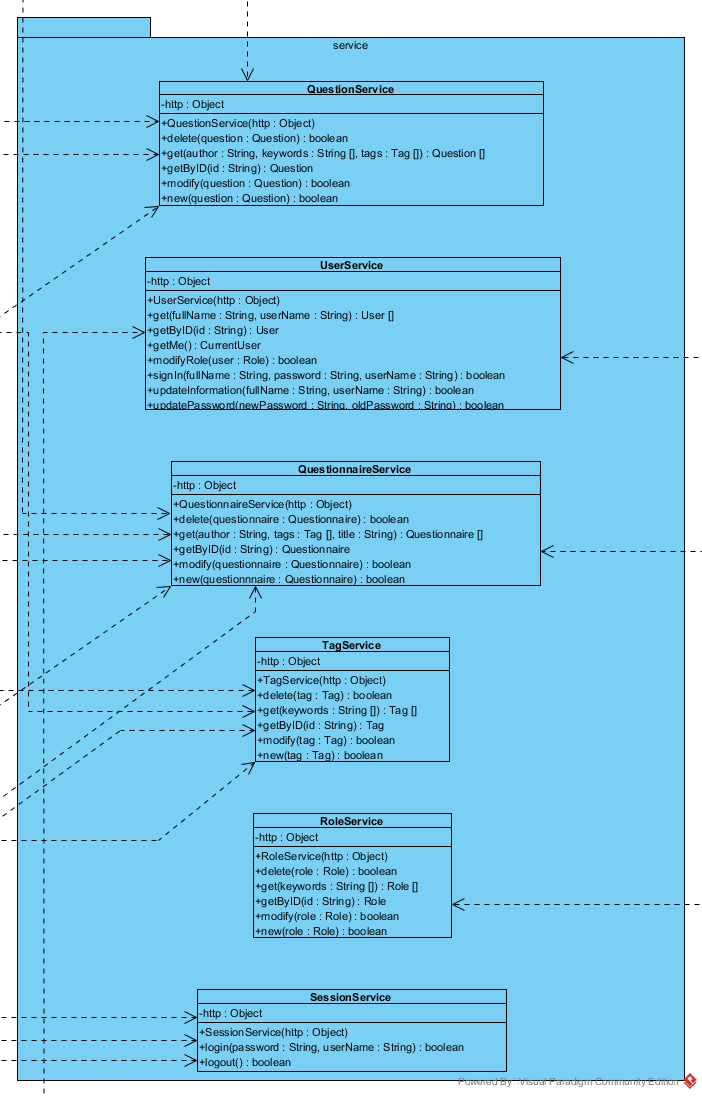
\includegraphics[scale=4, max width=\textwidth, max height=\myheight]{../img/diagrammiClassi/client/model/service.png}
		\caption{Diagramma package - client::model::service}
	\end{figure}
\end{center}\hypertarget{client::model::service::SessionService}{}
\subsubsubsection[SessionService]{client::model::service::SessionService}
\begin{figure}[H]
	\centering
	\begin{tikzpicture}
	\umlclass{client::model::service::SessionService} {--http : \$http\\--configuration : Configuration}{+SessionService(http : Object, configuration : Configuration)\\+login(password : String, userName : String, next : Function, err : Function) : void\\+logout(next : Function, err : Function) : void}
	\end{tikzpicture}
	\caption{Diagramma classe - client::model::service::SessionService}
\end{figure}\begin{description}
\item[Descrizione] \hfill \\
Questa classe fornisce al client i servizi relativi  alle credenziali d'accesso di un utente utilizzando chiamate HTTP all'end-point /api/session
\item[Relazioni con altre classi] \hfill \\
\vspace{-7mm}
\begin{description}
	\item[\hyperlink{client::controller::public::LogIn}{client::controller::public::LogIn}] \hfill \\
	Relazione entrante, campo dati che rappresenta un oggetto SessionService
	\item[\hyperlink{client::controller::user::Home}{client::controller::user::Home}] \hfill \\
	Relazione entrante, campo dati che rappresenta un oggetto SessionService
	\item[\hyperlink{client::app::Configuration}{client::app::Configuration}] \hfill \\
	Relazione uscente, campo dati che rappresenta un oggetto Configuration
	\item[\hyperlink{client::controller::public::SignUp}{client::controller::public::SignUp}] \hfill \\
	Relazione entrante, campo dati che rappresenta un oggetto SessionService
\end{description}

\item[Attributi] \hfill \\
\vspace{-7mm}
\begin{itemize}
	\item http : \$http $\rightarrow$ oggetto del servizio offerto da angulajs per le richieste http
	\item configuration : Configuration $\rightarrow$ campo dati che rappresenta un oggetto Configuration
\end{itemize}

\item[Metodi] \hfill \\
\vspace{-7mm}
\begin{itemize}
	\item SessionService(http : Object, configuration : Configuration) $\rightarrow$ costruttore della classe\begin{itemize}
		\item http $\rightarrow$ oggetto del servizio offerto da angulajs per le richieste http
		\item configuration $\rightarrow$ campo dati che rappresenta un oggetto Configuration
	\end{itemize}
	
	\item login(password : String, userName : String, next : Function, err : Function) : void $\rightarrow$ provvede ad effettuare l'accesso presso il server\begin{itemize}
		\item password $\rightarrow$ contiene la password inserita dall'utente
		\item userName $\rightarrow$ contiene l'username inserito dall'utente
		\item next $\rightarrow$ questo parametro rappresenta la callback che il metodo chiama in caso di successo
		\item err $\rightarrow$ questo parametro rappresenta la callback che il metodo chiama in caso di errore
	\end{itemize}
	
	\item logout(next : Function, err : Function) : void $\rightarrow$ chiude la sessione dell'utente\begin{itemize}
		\item next $\rightarrow$ questo parametro rappresenta la callback che il metodo chiama in caso di successo
		\item err $\rightarrow$ questo parametro rappresenta la callback che il metodo chiama in caso di errore
	\end{itemize}
	
\end{itemize}

\end{description}

\vspace{0.5cm}
\hypertarget{client::model::service::UserService}{}
\subsubsubsection[UserService]{client::model::service::UserService}
\begin{figure}[H]
	\centering
	\begin{tikzpicture}
	\umlclass{client::model::service::UserService} {--http : \$http\\--configuration : Configuration\\--roleService : RoleService}{+UserService(http : Object)\\+get(fullName : String[], userName : String[], next : Function, err : Function) : void\\+getByID(id : String, next : Function, err : Function) : void\\+getMe(next : Function, err : Function) : void\\+signUp(fullName : String, password : String, userName : String, next : Function, err : Function) : void\\+updateInformation(fullName : String, userName : String, next : Function, err : Function) : void\\+updatePassword(newPassword : String, oldPassword : String, next : Function, err : Function) : void\\+modifyRole(user : User, role : Role, next : Function, err : Function) : void\\+delete(user : User, next : Function, err : Function) : void}
	\end{tikzpicture}
	\caption{Diagramma classe - client::model::service::UserService}
\end{figure}\begin{description}
\item[Descrizione] \hfill \\
Questa classe fornisce al client i servizi relativi al profilo, utilizzando chiamate HTTP agli end-point /api/users e /api/roles
\item[Relazioni con altre classi] \hfill \\
\vspace{-7mm}
\begin{description}
	\item[\hyperlink{client::controller::public::LogIn}{client::controller::public::LogIn}] \hfill \\
	Relazione entrante, campo dati che rappresenta un oggetto UserService
	\item[\hyperlink{client::controller::user::User}{client::controller::user::User}] \hfill \\
	Relazione entrante, campo dati che rappresenta un oggetto UserService
	\item[\hyperlink{client::app::Configuration}{client::app::Configuration}] \hfill \\
	Relazione uscente, campo dati che rappresenta un oggetto Configuration
	\item[\hyperlink{client::model::service::RoleService}{client::model::service::RoleService}] \hfill \\
	Relazione uscente, campo dati che rappresenta un oggetto RoleService
	\item[\hyperlink{client::controller::student::Questionnaires}{client::controller::student::Questionnaires}] \hfill \\
	Relazione entrante, campo dati che rappresenta un oggetto UserService
	\item[\hyperlink{client::controller::teacher::ManipulateQuestionnaire}{client::controller::teacher::ManipulateQuestionnaire}] \hfill \\
	Relazione entrante, campo dati che rappresenta un oggetto UserService
	\item[\hyperlink{client::controller::teacher::SelectQuestion}{client::controller::teacher::SelectQuestion}] \hfill \\
	Relazione entrante, campo dati che rappresenta un oggetto UserService
	\item[\hyperlink{client::controller::public::SignUp}{client::controller::public::SignUp}] \hfill \\
	Relazione entrante, campo dati che rappresenta un oggetto UserService
	\item[\hyperlink{client::controller::public::Home}{client::controller::public::Home}] \hfill \\
	Relazione entrante, campo dati che rappresenta un oggetto UserService
	\item[\hyperlink{client::controller::admin::UsersList}{client::controller::admin::UsersList}] \hfill \\
	Relazione entrante, campo dati che rappresenta un oggetto UserService
\end{description}

\item[Attributi] \hfill \\
\vspace{-7mm}
\begin{itemize}
	\item http : \$http $\rightarrow$ oggetto del servizio offerto da angulajs per le richieste http
	\item configuration : Configuration $\rightarrow$ campo dati che rappresenta un oggetto Configuration
	\item roleService : RoleService $\rightarrow$ campo dati che rappresenta un oggetto RoleService
\end{itemize}

\item[Metodi] \hfill \\
\vspace{-7mm}
\begin{itemize}
	\item UserService(http : Object) $\rightarrow$ costruttore della classe\begin{itemize}
		\item http $\rightarrow$ oggetto del servizio offerto da angulajs per le richieste http
	\end{itemize}
	
	\item get(fullName : String[], userName : String[], next : Function, err : Function) : void $\rightarrow$ tramite API REST ritorna una lista di utenti sul server filtrate in base ai parametri\begin{itemize}
		\item fullName $\rightarrow$ contiene il nome del utente da ricercare 
		\item userName $\rightarrow$ contiene il username dell'utente da ricercare 
		\item next $\rightarrow$ questo parametro rappresenta la callback che il metodo chiama in caso di successo
		\item err $\rightarrow$ questo parametro rappresenta la callback che il metodo chiama in caso di errore
	\end{itemize}
	
	\item getByID(id : String, next : Function, err : Function) : void $\rightarrow$ tramite API REST ritorna un utente dal server per ID\begin{itemize}
		\item id $\rightarrow$ contiene id dell'utente da ricercare 
		\item next $\rightarrow$ questo parametro rappresenta la callback che il metodo chiama in caso di successo
		\item err $\rightarrow$ questo parametro rappresenta la callback che il metodo chiama in caso di errore
	\end{itemize}
	
	\item getMe(next : Function, err : Function) : void $\rightarrow$ tramite API REST ritorna l'utente corrente\begin{itemize}
		\item next $\rightarrow$ questo parametro rappresenta la callback che il metodo chiama in caso di successo
		\item err $\rightarrow$ questo parametro rappresenta la callback che il metodo chiama in caso di errore
	\end{itemize}
	
	\item signUp(fullName : String, password : String, userName : String, next : Function, err : Function) : void $\rightarrow$ tramite API REST crea un nuovo utente sul server\begin{itemize}
		\item fullName $\rightarrow$ contiene il nome del nuovo utente
		\item password $\rightarrow$ contiene la password del nuovo utente
		\item userName $\rightarrow$ contiene il username del nuovo utente
		\item next $\rightarrow$ questo parametro rappresenta la callback che il metodo chiama in caso di successo
		\item err $\rightarrow$ questo parametro rappresenta la callback che il metodo chiama in caso di errore
	\end{itemize}
	
	\item updateInformation(fullName : String, userName : String, next : Function, err : Function) : void $\rightarrow$ tramite API REST modifica le informazioni di profilo dell'utente corrente sul server\begin{itemize}
		\item fullName $\rightarrow$ contiene il nuovo nome dell'utente
		\item userName $\rightarrow$ contiene il nuovo username dell'utente
		\item next $\rightarrow$ questo parametro rappresenta la callback che il metodo chiama in caso di successo
		\item err $\rightarrow$ questo parametro rappresenta la callback che il metodo chiama in caso di errore
	\end{itemize}
	
	\item updatePassword(newPassword : String, oldPassword : String, next : Function, err : Function) : void $\rightarrow$ tramite API REST modifica la password dell'utente corrente sul server\begin{itemize}
		\item newPassword $\rightarrow$ contiene il nuovo password dell'utente
		\item oldPassword $\rightarrow$ contiene la vecchia password dell'utente
		\item next $\rightarrow$ questo parametro rappresenta la callback che il metodo chiama in caso di successo
		\item err $\rightarrow$ questo parametro rappresenta la callback che il metodo chiama in caso di errore
	\end{itemize}
	
	\item modifyRole(user : User, role : Role, next : Function, err : Function) : void $\rightarrow$ tramite API REST modifica il ruolo dell'utente corrente sul server\begin{itemize}
		\item user $\rightarrow$ contiene l'utente il cui ruolo deve essere cambiato
		\item role $\rightarrow$ contiene il nuovo ruolo dell'utente
		\item next $\rightarrow$ questo parametro rappresenta la callback che il metodo chiama in caso di successo
		\item err $\rightarrow$ questo parametro rappresenta la callback che il metodo chiama in caso di errore
	\end{itemize}
	
	\item delete(user : User, next : Function, err : Function) : void $\rightarrow$ tramite API REST elimina un utente sul server\begin{itemize}
		\item user $\rightarrow$ 
		\item next $\rightarrow$ questo parametro rappresenta la callback che il metodo chiama in caso di successo
		\item err $\rightarrow$ questo parametro rappresenta la callback che il metodo chiama in caso di errore
	\end{itemize}
	
\end{itemize}

\end{description}

\vspace{0.5cm}
\hypertarget{client::model::service::TagService}{}
\subsubsubsection[TagService]{client::model::service::TagService}
\begin{figure}[H]
	\centering
	\begin{tikzpicture}
	\umlclass{client::model::service::TagService} {--http : \$http\\--configuration : Configuration}{+TagService(http : Object, configuration : Configuration)\\+delete(tag : Tag, next : Function, err : Function) : void\\+get(keywords : String[], next : Function, err : Function) : void\\+getByID(id : String, next : Function, err : Function) : void\\+modify(tag : Tag, next : Function, err : Function) : void\\+new(tag : Tag, next : Function, err : Function) : void}
	\end{tikzpicture}
	\caption{Diagramma classe - client::model::service::TagService}
\end{figure}\begin{description}
\item[Descrizione] \hfill \\
Questa classe fornisce al client i servizi relativi alla modifica, cancellazione e lettura e inserimento dei tag presenti nel sistema, utilizzando chiamate HTTP all'end-point /api/tags
\item[Relazioni con altre classi] \hfill \\
\vspace{-7mm}
\begin{description}
	\item[\hyperlink{client::app::Configuration}{client::app::Configuration}] \hfill \\
	Relazione uscente, campo dati che rappresenta un oggetto Configuration
	\item[\hyperlink{client::controller::teacher::ManageQuestionnaires}{client::controller::teacher::ManageQuestionnaires}] \hfill \\
	Relazione entrante, campo dati che rappresenta un oggetto TagService
	\item[\hyperlink{client::controller::teacher::ManageQuestions}{client::controller::teacher::ManageQuestions}] \hfill \\
	Relazione entrante, campo dati che rappresenta un oggetto TagService
	\item[\hyperlink{client::controller::teacher::ManipulateQuestion}{client::controller::teacher::ManipulateQuestion}] \hfill \\
	Relazione entrante, campo dati che rappresenta un oggetto TagService
	\item[\hyperlink{client::controller::teacher::ManipulateQuestionnaire}{client::controller::teacher::ManipulateQuestionnaire}] \hfill \\
	Relazione entrante, campo dati che rappresenta un oggetto TagService
	\item[\hyperlink{client::controller::teacher::SelectQuestion}{client::controller::teacher::SelectQuestion}] \hfill \\
	Relazione entrante, campo dati che rappresenta un oggetto TagService
	\item[\hyperlink{client::controller::student::Questionnaires}{client::controller::student::Questionnaires}] \hfill \\
	Relazione entrante, campo dati che rappresenta un oggetto TagService
	\item[\hyperlink{client::controller::teacher::ManageTags}{client::controller::teacher::ManageTags}] \hfill \\
	Relazione entrante, campo dati che rappresenta un oggetto TagService
\end{description}

\item[Attributi] \hfill \\
\vspace{-7mm}
\begin{itemize}
	\item http : \$http $\rightarrow$ oggetto del servizio offerto da angulajs per le richieste http
	\item configuration : Configuration $\rightarrow$ campo dati che rappresenta un oggetto Configuration
\end{itemize}

\item[Metodi] \hfill \\
\vspace{-7mm}
\begin{itemize}
	\item TagService(http : Object, configuration : Configuration) $\rightarrow$ costruttore della classe\begin{itemize}
		\item http $\rightarrow$ oggetto del servizio offerto da angulajs per le richieste http
		\item configuration $\rightarrow$ campo dati che rappresenta un oggetto Configuration
	\end{itemize}
	
	\item delete(tag : Tag, next : Function, err : Function) : void $\rightarrow$ tramite API REST elimina un argomento sul server\begin{itemize}
		\item tag $\rightarrow$ contiene l'argomento da eliminare
		\item next $\rightarrow$ questo parametro rappresenta la callback che il metodo chiama in caso di successo
		\item err $\rightarrow$ questo parametro rappresenta la callback che il metodo chiama in caso di errore
	\end{itemize}
	
	\item get(keywords : String[], next : Function, err : Function) : void $\rightarrow$ tramite API REST ritorna una lista di argomenti sul server filtrate in base ai parametri\begin{itemize}
		\item keywords $\rightarrow$ contiene la lista di parole chiave per ricercare gli argomenti
		\item next $\rightarrow$ questo parametro rappresenta la callback che il metodo chiama in caso di successo
		\item err $\rightarrow$ questo parametro rappresenta la callback che il metodo chiama in caso di errore
	\end{itemize}
	
	\item getByID(id : String, next : Function, err : Function) : void $\rightarrow$ tramite API REST ritorna un argomento dal server per ID\begin{itemize}
		\item id $\rightarrow$ contiene id dell'argomento da ricercare
		\item next $\rightarrow$ questo parametro rappresenta la callback che il metodo chiama in caso di successo
		\item err $\rightarrow$ questo parametro rappresenta la callback che il metodo chiama in caso di errore
	\end{itemize}
	
	\item modify(tag : Tag, next : Function, err : Function) : void $\rightarrow$ tramite API REST modifica un argomento sul server\begin{itemize}
		\item tag $\rightarrow$ contiene l'argomento da modificare
		\item next $\rightarrow$ questo parametro rappresenta la callback che il metodo chiama in caso di successo
		\item err $\rightarrow$ questo parametro rappresenta la callback che il metodo chiama in caso di errore
	\end{itemize}
	
	\item new(tag : Tag, next : Function, err : Function) : void $\rightarrow$ tramite API REST crea un nuovo argomento sul server\begin{itemize}
		\item tag $\rightarrow$ contiene il nuovo argomento da creare
		\item next $\rightarrow$ questo parametro rappresenta la callback che il metodo chiama in caso di successo
		\item err $\rightarrow$ questo parametro rappresenta la callback che il metodo chiama in caso di errore
	\end{itemize}
	
\end{itemize}

\end{description}

\vspace{0.5cm}
\hypertarget{client::model::service::RoleService}{}
\subsubsubsection[RoleService]{client::model::service::RoleService}
\begin{figure}[H]
	\centering
	\begin{tikzpicture}
	\umlclass{client::model::service::RoleService} {--http : \$http\\--configuration : Configuration}{+RoleService(http : Object, configuration : Configuration)\\+get(keywords : String[], next : Function, err : Function) : void\\+getByID(id : String, next : Function, err : Function) : void}
	\end{tikzpicture}
	\caption{Diagramma classe - client::model::service::RoleService}
\end{figure}\begin{description}
\item[Descrizione] \hfill \\
Questa classe fornisce al client i servizi necessari per la gestione dei ruoli, utilizzando chiamate HTTP all'end-point /api/tags
\item[Relazioni con altre classi] \hfill \\
\vspace{-7mm}
\begin{description}
	\item[\hyperlink{client::model::service::UserService}{client::model::service::UserService}] \hfill \\
	Relazione entrante, campo dati che rappresenta un oggetto RoleService
	\item[\hyperlink{client::app::Configuration}{client::app::Configuration}] \hfill \\
	Relazione uscente, campo dati che rappresenta un oggetto Configuration
	\item[\hyperlink{client::controller::admin::UsersList}{client::controller::admin::UsersList}] \hfill \\
	Relazione entrante, campo dati che rappresenta un oggetto RoleService
\end{description}

\item[Attributi] \hfill \\
\vspace{-7mm}
\begin{itemize}
	\item http : \$http $\rightarrow$ oggetto del servizio offerto da angulajs per le richieste http
	\item configuration : Configuration $\rightarrow$ campo dati che rappresenta un oggetto Configuration
\end{itemize}

\item[Metodi] \hfill \\
\vspace{-7mm}
\begin{itemize}
	\item RoleService(http : Object, configuration : Configuration) $\rightarrow$ costruttore della classe\begin{itemize}
		\item http $\rightarrow$ oggetto del servizio offerto da angulajs per le richieste http
		\item configuration $\rightarrow$ campo dati che rappresenta un oggetto Configuration
	\end{itemize}
	
	\item get(keywords : String[], next : Function, err : Function) : void $\rightarrow$ tramite API REST ritorna una lista dei ruoli sul server filtrate in base ai parametri\begin{itemize}
		\item keywords $\rightarrow$ contiene la lista di parole chiave per ricercare il ruolo
		\item next $\rightarrow$ questo parametro rappresenta la callback che il metodo chiama in caso di successo
		\item err $\rightarrow$ questo parametro rappresenta la callback che il metodo chiama in caso di errore
	\end{itemize}
	
	\item getByID(id : String, next : Function, err : Function) : void $\rightarrow$ tramite API REST ritorna un ruolo dal server per ID\begin{itemize}
		\item id $\rightarrow$ contiene id del ruolo da ricercare
		\item next $\rightarrow$ questo parametro rappresenta la callback che il metodo chiama in caso di successo
		\item err $\rightarrow$ questo parametro rappresenta la callback che il metodo chiama in caso di errore
	\end{itemize}
	
\end{itemize}

\end{description}

\vspace{0.5cm}
\hypertarget{client::model::service::QuestionService}{}
\subsubsubsection[QuestionService]{client::model::service::QuestionService}
\begin{figure}[H]
	\centering
	\begin{tikzpicture}
	\umlclass{client::model::service::QuestionService} {--http : \$http\\--configuration : Configuration}{+QuestionService(http : Object, configuration : Configuration)\\+delete(question : Question, next : Function, err : Function) : void\\+get(author : String[], keywords : String[], tags : String[], next : Function, err : Function) : void\\+getByID(id : String, next : Function, err : Function) : void\\+modify(question : Question, next : Function, err : Function) : void\\+new(question : Question, next : Function, err : Function) : void}
	\end{tikzpicture}
	\caption{Diagramma classe - client::model::service::QuestionService}
\end{figure}\begin{description}
\item[Descrizione] \hfill \\
Questa classe fornisce al client i servizi necessari alla gestione delle domande, utilizzando chiamate HTTP all'end-point /api/questions
\item[Relazioni con altre classi] \hfill \\
\vspace{-7mm}
\begin{description}
	\item[\hyperlink{client::app::Configuration}{client::app::Configuration}] \hfill \\
	Relazione uscente, campo dati che rappresenta un oggetto Configuration
	\item[\hyperlink{client::controller::teacher::ManipulateQuestionnaire}{client::controller::teacher::ManipulateQuestionnaire}] \hfill \\
	Relazione entrante, campo dati che rappresenta un oggetto QuestionService
	\item[\hyperlink{client::controller::teacher::ManipulateQuestion}{client::controller::teacher::ManipulateQuestion}] \hfill \\
	Relazione entrante, campo dati che rappresenta un oggetto QuestionService
	\item[\hyperlink{client::controller::teacher::SelectQuestion}{client::controller::teacher::SelectQuestion}] \hfill \\
	Relazione entrante, campo dati che rappresenta un oggetto QuestionService
	\item[\hyperlink{client::controller::teacher::ManageQuestions}{client::controller::teacher::ManageQuestions}] \hfill \\
	Relazione entrante, campo dati che rappresenta un oggetto QuestionService
\end{description}

\item[Attributi] \hfill \\
\vspace{-7mm}
\begin{itemize}
	\item http : \$http $\rightarrow$ oggetto del servizio offerto da angulajs per le richieste http
	\item configuration : Configuration $\rightarrow$ campo dati che rappresenta un oggetto Configuration
\end{itemize}

\item[Metodi] \hfill \\
\vspace{-7mm}
\begin{itemize}
	\item QuestionService(http : Object, configuration : Configuration) $\rightarrow$ costruttore della classe\begin{itemize}
		\item http $\rightarrow$ oggetto del servizio offerto da angulajs per le richieste http
		\item configuration $\rightarrow$ campo dati che rappresenta un oggetto Configuration
	\end{itemize}
	
	\item delete(question : Question, next : Function, err : Function) : void $\rightarrow$ tramite API REST elimina una domanda sul server\begin{itemize}
		\item question $\rightarrow$ contiene la domanda da eliminare
		\item next $\rightarrow$ questo parametro rappresenta la callback che il metodo chiama in caso di successo
		\item err $\rightarrow$ questo parametro rappresenta la callback che il metodo chiama in caso di errore
	\end{itemize}
	
	\item get(author : String[], keywords : String[], tags : String[], next : Function, err : Function) : void $\rightarrow$ tramite API REST ritorna una lista delle domande sul server filtrate in base ai parametri\begin{itemize}
		\item author $\rightarrow$ contiene il nome dell'autore della domanda da ricercare 
		\item keywords $\rightarrow$ contiene la lista di parole chiave per ricercare una domanda
		\item tags $\rightarrow$ contiene la lista degli argomenti per ricercare una domanda
		\item next $\rightarrow$ questo parametro rappresenta la callback che il metodo chiama in caso di successo
		\item err $\rightarrow$ questo parametro rappresenta la callback che il metodo chiama in caso di errore
	\end{itemize}
	
	\item getByID(id : String, next : Function, err : Function) : void $\rightarrow$ tramite API REST ritorna una domanda dal server per ID\begin{itemize}
		\item id $\rightarrow$ ID della Question
		\item next $\rightarrow$ questo parametro rappresenta la callback che il metodo chiama in caso di successo
		\item err $\rightarrow$ questo parametro rappresenta la callback che il metodo chiama in caso di errore
	\end{itemize}
	
	\item modify(question : Question, next : Function, err : Function) : void $\rightarrow$ tramite API REST modifica una domanda sul server\begin{itemize}
		\item question $\rightarrow$ contiene la domanda da modificare
		\item next $\rightarrow$ questo parametro rappresenta la callback che il metodo chiama in caso di successo
		\item err $\rightarrow$ questo parametro rappresenta la callback che il metodo chiama in caso di errore
	\end{itemize}
	
	\item new(question : Question, next : Function, err : Function) : void $\rightarrow$ tramite API REST crea una nuova domanda sul server\begin{itemize}
		\item question $\rightarrow$ contiene la nuova domanda da creare
		\item next $\rightarrow$ questo parametro rappresenta la callback che il metodo chiama in caso di successo
		\item err $\rightarrow$ questo parametro rappresenta la callback che il metodo chiama in caso di errore
	\end{itemize}
	
\end{itemize}

\end{description}

\vspace{0.5cm}
\hypertarget{client::model::service::QuestionnaireService}{}
\subsubsubsection[QuestionnaireService]{client::model::service::QuestionnaireService}
\begin{figure}[H]
	\centering
	\begin{tikzpicture}
	\umlclass{client::model::service::QuestionnaireService} {--http : \$http\\--configuration : Configuration}{+QuestionnaireService(http : Object, configuration : Configuration)\\+delete(questionnaire : Questionnaire, next : Function, err : Function) : void\\+get (author : String[], tags  : String[], title : String[], next : Function, err : Function) : void\\+getByID(id : String, next : Function, err : Function) : void\\+modify(questionnaire : Questionnaire, next : Function, err : Function) : void\\+new(questionnaire : Questionnaire, next : Function, err : Function) : void}
	\end{tikzpicture}
	\caption{Diagramma classe - client::model::service::QuestionnaireService}
\end{figure}\begin{description}
\item[Descrizione] \hfill \\
Questa classe fornisce al client i servizi necessari alla gestione dei questionari, utilizzando chiamate HTTP all'end-point /api/questionnaires
\item[Relazioni con altre classi] \hfill \\
\vspace{-7mm}
\begin{description}
	\item[\hyperlink{client::app::Configuration}{client::app::Configuration}] \hfill \\
	Relazione uscente, campo dati che rappresenta un oggetto Configuration
	\item[\hyperlink{client::controller::student::Questionnaires}{client::controller::student::Questionnaires}] \hfill \\
	Relazione entrante, campo dati che rappresenta un oggetto QuestionnaireService
	\item[\hyperlink{client::controller::student::ExecuteQuestionnaire}{client::controller::student::ExecuteQuestionnaire}] \hfill \\
	Relazione entrante, campo dati che rappresenta un oggetto QuestionnaireService
	\item[\hyperlink{client::controller::teacher::ManipulateQuestionnaire}{client::controller::teacher::ManipulateQuestionnaire}] \hfill \\
	Relazione entrante, campo dati che rappresenta un oggetto QuestionnaireService
	\item[\hyperlink{client::controller::teacher::ManageQuestionnaires}{client::controller::teacher::ManageQuestionnaires}] \hfill \\
	Relazione entrante, campo dati che rappresenta un oggetto QuestionnaireService
\end{description}

\item[Attributi] \hfill \\
\vspace{-7mm}
\begin{itemize}
	\item http : \$http $\rightarrow$ oggetto del servizio offerto da angulajs per le richieste http
	\item configuration : Configuration $\rightarrow$ campo dati che rappresenta un oggetto Configuration
\end{itemize}

\item[Metodi] \hfill \\
\vspace{-7mm}
\begin{itemize}
	\item QuestionnaireService(http : Object, configuration : Configuration) $\rightarrow$ costruttore della classe\begin{itemize}
		\item http $\rightarrow$ oggetto del servizio offerto da angulajs per le richieste http
		\item configuration $\rightarrow$ campo dati che rappresenta un oggetto Configuration
	\end{itemize}
	
	\item delete(questionnaire : Questionnaire, next : Function, err : Function) : void $\rightarrow$ tramite API REST elimina un questionario sul server\begin{itemize}
		\item questionnaire $\rightarrow$ contiene il questionario da eliminare
		\item next $\rightarrow$ questo parametro rappresenta la callback che il metodo chiama in caso di successo
		\item err $\rightarrow$ questo parametro rappresenta la callback che il metodo chiama in caso di errore
	\end{itemize}
	
	\item get (author : String[], tags  : String[], title : String[], next : Function, err : Function) : void $\rightarrow$ tramite API REST ritorna una lista di questionari sul server filtrate in base ai parametri\begin{itemize}
		\item author $\rightarrow$ contiene il nome dell'autore del questionario da ricercare
		\item tags  $\rightarrow$ contiene la lista degli argomenti per ricercare un questionario
		\item title $\rightarrow$ contiene il titolo del questionario da ricercare
		\item next $\rightarrow$ questo parametro rappresenta la callback che il metodo chiama in caso di successo
		\item err $\rightarrow$ questo parametro rappresenta la callback che il metodo chiama in caso di errore
	\end{itemize}
	
	\item getByID(id : String, next : Function, err : Function) : void $\rightarrow$ tramite API REST ritorna un questionario dal server per ID\begin{itemize}
		\item id $\rightarrow$ contiene id del questionario da ricercare
		\item next $\rightarrow$ questo parametro rappresenta la callback che il metodo chiama in caso di successo
		\item err $\rightarrow$ questo parametro rappresenta la callback che il metodo chiama in caso di errore
	\end{itemize}
	
	\item modify(questionnaire : Questionnaire, next : Function, err : Function) : void $\rightarrow$ tramite API REST modifica un questionario sul server\begin{itemize}
		\item questionnaire $\rightarrow$ contiene il questionario da modificare
		\item next $\rightarrow$ questo parametro rappresenta la callback che il metodo chiama in caso di successo
		\item err $\rightarrow$ questo parametro rappresenta la callback che il metodo chiama in caso di errore
	\end{itemize}
	
	\item new(questionnaire : Questionnaire, next : Function, err : Function) : void $\rightarrow$ tramite API REST crea un nuovo questionario sul server\begin{itemize}
		\item questionnaire $\rightarrow$ contiene il nuovo questionario da creare
		\item next $\rightarrow$ questo parametro rappresenta la callback che il metodo chiama in caso di successo
		\item err $\rightarrow$ questo parametro rappresenta la callback che il metodo chiama in caso di errore
	\end{itemize}
	
\end{itemize}

\end{description}

\vspace{0.5cm}
\hypertarget{client::model::service::AnswerService}{}
\subsubsubsection[AnswerService]{client::model::service::AnswerService}
\begin{figure}[H]
	\centering
	\begin{tikzpicture}
	\umlclass{client::model::service::AnswerService} {--configuration : Configuration\\--http : \$http}{+AnswerService(configuration : Configuration, http : Object)\\+get(next : Function, err : Function, author : String[], question : Question	, questionnaire : Questionnaire) : void\\+new(next : Function, err : Function, questionnaire : Questionnaire, question : Question	, score : double) : void}
	\end{tikzpicture}
	\caption{Diagramma classe - client::model::service::AnswerService}
\end{figure}\begin{description}
\item[Descrizione] \hfill \\
Questa classe fornisce al client i servizi necessari alla gestione delle statistiche, utilizzando chiamate HTTP all'end-point /api/answers
\item[Relazioni con altre classi] \hfill \\
\vspace{-7mm}
\begin{description}
	\item[\hyperlink{client::app::Configuration}{client::app::Configuration}] \hfill \\
	Relazione uscente, campo dati che rappresenta un oggetto Configuration
	\item[\hyperlink{client::controller::student::ExecuteQuestionnaire}{client::controller::student::ExecuteQuestionnaire}] \hfill \\
	Relazione entrante, campo dati che rappresenta un oggetto AnswerService	
	\item[\hyperlink{client::controller::user::Welcome}{client::controller::user::Welcome}] \hfill \\
	Relazione entrante, campo dati che rappresenta un oggetto AnswerService
\end{description}

\item[Attributi] \hfill \\
\vspace{-7mm}
\begin{itemize}
	\item configuration : Configuration $\rightarrow$ campo dati che rappresenta un oggetto Configuration
	\item http : \$http $\rightarrow$ oggetto del servizio offerto da angulajs per le richieste http	
\end{itemize}

\item[Metodi] \hfill \\
\vspace{-7mm}
\begin{itemize}
	\item AnswerService(configuration : Configuration, http : Object) $\rightarrow$ costruttore della classe\begin{itemize}
		\item configuration $\rightarrow$ campo dati che rappresenta un oggetto Configuration	
		\item http $\rightarrow$ oggetto del servizio offerto da angulajs per le richieste http	
	\end{itemize}
	
	\item get(next : Function, err : Function, author : String[], question : Question	, questionnaire : Questionnaire) : void $\rightarrow$ tramite API REST ritorna una lista di questionari sul server filtrate in base ai parametri	\begin{itemize}
		\item next $\rightarrow$ questo parametro rappresenta la callback che il metodo chiama in caso di successo
		\item err $\rightarrow$ questo parametro rappresenta la callback che il metodo chiama in caso di errore	
		\item author $\rightarrow$ contiene il nome dell'autore del questionario da ricercare
		\item question $\rightarrow$ contiene la domanda a cui l'utente ha risposto
		\item questionnaire $\rightarrow$ contiene il questionario che l'utente ha eseguito
	\end{itemize}
	
	\item new(next : Function, err : Function, questionnaire : Questionnaire, question : Question	, score : double) : void $\rightarrow$ tramite API REST crea una nuova risposta ad una domanda sul server
	\begin{itemize}
		\item next $\rightarrow$ questo parametro rappresenta la callback che il metodo chiama in caso di successo
		\item err $\rightarrow$ questo parametro rappresenta la callback che il metodo chiama in caso di errore
		\item questionnaire $\rightarrow$ contiene il questionario che l'utente ha eseguito
		\item question $\rightarrow$ contiene la domanda a cui l'utente ha risposto
		\item score $\rightarrow$ contiene il punteggio che l'utente ha totalizzato sulla singola domanda risposta
	\end{itemize}
	
\end{itemize}

\end{description}

\vspace{0.5cm}
\subsection{client::controller}
È il package che contiene le componenti che contengono i
controller dell’applicazione e che incapsulano le funzionalità di two-way data binding tra le View e il Model. In esse è contenuta la logica applicativa riguardante le diverse pagine HTML.\begin{center}
	\begin{figure}[H]
		\centering 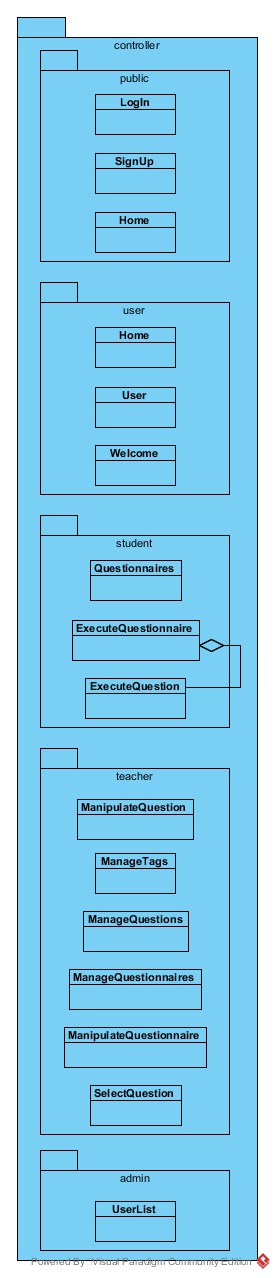
\includegraphics[scale=4, max width=\textwidth, max height=\myheight]{../img/diagrammiClassi/client/controller.png}
		\caption{Diagramma package - client::controller}
	\end{figure}
\end{center}\subsubsection{client::controller::public}
È il package che contiene tutte le classi che costituiscono i controller della porzione pubblica di un client. Ogni componente si occupa della gestione di una particolare porzione dell'interfaccia di un utente non autenticato che verrà successivamente visualizzata nella corrispondente view.\begin{center}
	\begin{figure}[H]
		\centering 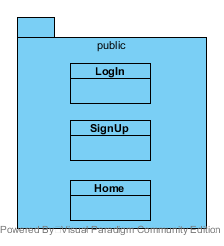
\includegraphics[scale=4, max width=\textwidth, max height=\myheight]{../img/diagrammiClassi/client/controller/public.png}
		\caption{Diagramma package - client::controller::public}
	\end{figure}
\end{center}\hypertarget{client::controller::public::LogIn}{}
\subsubsubsection[LogIn]{client::controller::public::LogIn}
\begin{figure}[H]
	\centering
	\begin{tikzpicture}
	\umlclass{client::controller::public::LogIn} {--location : \$location\\--rootScope : \$rootScope\\--scope : \$scope\\--sessionService : SessionService\\--check : Check\\--userService : UserService\\--cookies : \$cookies\\--error : Error\\--userName : String\\--password : String}{+LogIn(check : Check, cookies : Object, location : Object, userService : UserService, rootScope : Object, scope : Object, sessionService : SessionService)\\+submit() : void\\+checkUserName() : boolean\\+checkPassword() : boolean\\+getError() : Error\\+getUserName() : String\\+getPassword() : String\\+setError(error : Error) : void\\+setUserName(userName : String) : void\\+setPassword(password : String) : void}
	\end{tikzpicture}
	\caption{Diagramma classe - client::controller::public::LogIn}
\end{figure}\begin{description}
\item[Descrizione] \hfill \\
Classe che gestisce le operazioni e la logica applicativa riguardante la pagina di autenticazione sul client
\item[Utilizzo] \hfill \\
Viene utilizzata per generare la pagina di autenticazione all’applicazione. Prima della creazione della view viene effettuato un controllo sull’esistenza di una sessione utente. In caso positivo il controller si occuperà di visualizzare la home dell'utente loggato, altrimenti si procederà alla pagina di Login predefinita.
\item[Relazioni con altre classi] \hfill \\
\vspace{-7mm}
\begin{description}
	\item[\hyperlink{client::util::Check}{client::util::Check}] \hfill \\
	Relazione uscente, campo dati che rappresenta un oggetto Check
	\item[\hyperlink{client::model::service::UserService}{client::model::service::UserService}] \hfill \\
	Relazione uscente, campo dati che rappresenta un oggetto UserService
	\item[\hyperlink{client::model::data::Error}{client::model::data::Error}] \hfill \\
	Relazione uscente, campo dati che rappresenta un oggetto Error
	\item[\hyperlink{client::model::service::SessionService}{client::model::service::SessionService}] \hfill \\
	Relazione uscente, campo dati che rappresenta un oggetto SessionService
\end{description}

\item[Attributi] \hfill \\
\vspace{-7mm}
\begin{itemize}
	\item location : \$location $\rightarrow$ oggetto di angular che analizza l'URL nella barra degli indirizzi del browser e lo rende disponibile all'applicazione
	\item rootScope : \$rootScope $\rightarrow$ oggetto di angular che identifica l’elemento con attributo ng-app
	\item scope : \$scope $\rightarrow$ oggetto di angular che fa riferimento ad una porzione di model di pertinenza di uno specifico controller
	\item sessionService : SessionService $\rightarrow$ campo dati che rappresenta un oggetto SessionService
	\item check : Check $\rightarrow$ campo dati che rappresenta un oggetto Check
	\item userService : UserService $\rightarrow$ campo dati che rappresenta un oggetto UserService
	\item cookies : \$cookies $\rightarrow$ oggetto di angular che permette di manipolare i cookies
	\item error : Error $\rightarrow$ campo dati che rappresenta un oggetto Error
	\item userName : String $\rightarrow$ rappresenta il campo userName nella View
	\item password : String $\rightarrow$ rappresenta il campo password nella view
\end{itemize}

\item[Metodi] \hfill \\
\vspace{-7mm}
\begin{itemize}
	\item LogIn(check : Check, cookies : Object, location : Object, userService : UserService, rootScope : Object, scope : Object, sessionService : SessionService) $\rightarrow$ costruttore della classe\begin{itemize}
		\item check $\rightarrow$ campo dati che rappresenta un oggetto Check
		\item cookies $\rightarrow$ oggetto di angular che permette di manipolare i cookies
		\item location $\rightarrow$ oggetto di angular che analizza l'URL nella barra degli indirizzi del browser e lo rende disponibile all'applicazione
		\item userService $\rightarrow$ campo dati che rappresenta un oggetto UserService
		\item rootScope $\rightarrow$ oggetto di angular che identifica l’elemento con attributo ng-app
		\item scope $\rightarrow$ oggetto di angular che fa riferimento ad una porzione di model di pertinenza di uno specifico controller
		\item sessionService $\rightarrow$ campo dati che rappresenta un oggetto SessionService
	\end{itemize}
	
	\item submit() : void $\rightarrow$ invia lo username e la password dell'utente al servizio che effettua l'autenticazione istanziando una nuova sessione
	\item checkUserName() : boolean $\rightarrow$ metodo che controlla che l'userName inserito rispetti alcuni parametri richiamando il relativo metodo nella classe Check
	\item checkPassword() : boolean $\rightarrow$ metodo che controlla che la password inserita rispetti alcuni parametri richiamando il relativo metodo nella classe Check
	\item getError() : Error $\rightarrow$ metodo che restituisce il valore del campo dati error
	\item getUserName() : String $\rightarrow$ metodo che restituisce il valore del campo dati userName
	\item getPassword() : String $\rightarrow$ metodo che restituisce il valore del campo dati password
	\item setError(error : Error) : void $\rightarrow$ metodo che cambia il valore del campo dati error\begin{itemize}
		\item error $\rightarrow$ campo dati che rappresenta un oggetto Error
	\end{itemize}
	
	\item setUserName(userName : String) : void $\rightarrow$ metodo che cambia il valore del campo dati userName\begin{itemize}
		\item userName $\rightarrow$ rappresenta il campo userName nella View
	\end{itemize}
	
	\item setPassword(password : String) : void $\rightarrow$ metodo che cambia il valore del campo dati password\begin{itemize}
		\item password $\rightarrow$ rappresenta il campo password nella view
	\end{itemize}
	
\end{itemize}

\end{description}

\vspace{0.5cm}
\hypertarget{client::controller::public::SignUp}{}
\subsubsubsection[SignUp]{client::controller::public::SignUp}
\begin{figure}[H]
	\centering
	\begin{tikzpicture}
	\umlclass{client::controller::public::SignUp} {--location : \$location\\--rootScope : \$rootScope\\--scope : \$scope\\--sessionService : SessionService\\--userService : UserService\\--cookies : \$cookies\\--check : Check\\--error	 : Error	\\--userName : String\\--password : String\\--fullName : String\\--repeatPassword : String}{+SignUp(check : Check, cookies : Object, location : Object, scope : Object, rootScope : Object, sessionService : SessionService, userService : UserService)\\+checkPassword() : boolean\\+checkRepeatPassword() : boolean\\+checkUserName() : boolean\\+submit() : void\\+checkFullName() : boolean\\+getError	() : Error	\\+getUserName() : String\\+getPassword() : String\\+getFullName() : String\\+getRepeatPassword() : String\\+setError	(error	 : Error	) : void\\+setUserName(userName : String) : void\\+setPassword(password : String) : void\\+setFullName(fullName : String) : void\\+setRepeatPassword(repeatPassword : String) : void}
	\end{tikzpicture}
	\caption{Diagramma classe - client::controller::public::SignUp}
\end{figure}\begin{description}
\item[Descrizione] \hfill \\
Classe che gestisce le operazioni e la logica applicativa riguardante la pagina di Registrazione sul client
\item[Utilizzo] \hfill \\
Deve visualizzare campi per l’inserimento della mail, password, nome e cognome. Deve poter gestire l'eventuale caso di errore se la mail dello studente è già presente nel sistema. Inoltre deve poter gestire il caso in cui di la password dello studente non rispetta i parametri prestabiliti 
\item[Relazioni con altre classi] \hfill \\
\vspace{-7mm}
\begin{description}
	\item[\hyperlink{client::util::Check}{client::util::Check}] \hfill \\
	Relazione uscente, campo dati che rappresenta un oggetto Check
	\item[\hyperlink{client::model::data::Error}{client::model::data::Error}] \hfill \\
	Relazione uscente, oggetto che rappresenta un errore da visualizzare all'utente
	\item[\hyperlink{client::model::service::SessionService}{client::model::service::SessionService}] \hfill \\
	Relazione uscente, campo dati che rappresenta un oggetto SessionService
	\item[\hyperlink{client::model::service::UserService}{client::model::service::UserService}] \hfill \\
	Relazione uscente, campo dati che rappresenta un oggetto UserService
\end{description}

\item[Attributi] \hfill \\
\vspace{-7mm}
\begin{itemize}
	\item location : \$location $\rightarrow$ oggetto di angular che analizza l'URL nella barra degli indirizzi del browser e lo rende disponibile all'applicazione
	\item rootScope : \$rootScope $\rightarrow$ oggetto di angular che identifica l’elemento con attributo ng-app
	\item scope : \$scope $\rightarrow$ oggetto di angular che fa riferimento ad una porzione di model di pertinenza di uno specifico controller
	\item sessionService : SessionService $\rightarrow$ campo dati che rappresenta un oggetto SessionService
	\item userService : UserService $\rightarrow$ campo dati che rappresenta un oggetto UserService
	\item cookies : \$cookies $\rightarrow$ oggetto di angular che permette di manipolare i cookies
	\item check : Check $\rightarrow$ campo dati che rappresenta un oggetto Check
	\item error	 : Error	 $\rightarrow$ oggetto che rappresenta un errore da visualizzare all'utente
	\item userName : String $\rightarrow$ rappresenta il campo userName nella View
	\item password : String $\rightarrow$ rappresenta il campo password nella View
	\item fullName : String $\rightarrow$ rappresenta il campo fullName nella View
	\item repeatPassword : String $\rightarrow$ rappresenta il campo repeatPassword nella View
\end{itemize}

\item[Metodi] \hfill \\
\vspace{-7mm}
\begin{itemize}
	\item SignUp(check : Check, cookies : Object, location : Object, scope : Object, rootScope : Object, sessionService : SessionService, userService : UserService) $\rightarrow$ costruttore della classe\begin{itemize}
		\item check $\rightarrow$ campo dati che rappresenta un oggetto Check
		\item cookies $\rightarrow$ oggetto di angular che permette di manipolare i cookies
		\item location $\rightarrow$ oggetto di angular che analizza l'URL nella barra degli indirizzi del browser e lo rende disponibile all'applicazione
		\item scope $\rightarrow$ oggetto di angular che fa riferimento ad una porzione di model di pertinenza di uno specifico controller
		\item rootScope $\rightarrow$ oggetto di angular che identifica l’elemento con attributo ng-app
		\item sessionService $\rightarrow$ campo dati che rappresenta un oggetto SessionService
		\item userService $\rightarrow$ campo dati che rappresenta un oggetto UserService
	\end{itemize}
	
	\item checkPassword() : boolean $\rightarrow$ controlla se la password inserita ha i requisiti minimi richiamando il relativo metodo nella classe Check
	\item checkRepeatPassword() : boolean $\rightarrow$ controlla se la password è uguale a quella inserita nel campo "Ripeti password"
	\item checkUserName() : boolean $\rightarrow$ controlla su lo username ha i requisiti minimi richiamando il relativo metodo nella classe Check
	\item submit() : void $\rightarrow$ invia i dati dell'utente al servizio che effettua la registrazione
	\item checkFullName() : boolean $\rightarrow$ controlla se il nome inserito ha i requisiti minimi richiamando il relativo metodo nella classe Check
	\item getError	() : Error	 $\rightarrow$ metodo che restituisce il valore del campo dati error	
	\item getUserName() : String $\rightarrow$ metodo che restituisce il valore del campo dati userName
	\item getPassword() : String $\rightarrow$ metodo che restituisce il valore del campo dati password
	\item getFullName() : String $\rightarrow$ metodo che restituisce il valore del campo dati fullName
	\item getRepeatPassword() : String $\rightarrow$ metodo che restituisce il valore del campo dati repeatPassword
	\item setError	(error	 : Error	) : void $\rightarrow$ metodo che cambia il valore del campo dati error	\begin{itemize}
		\item error	 $\rightarrow$ oggetto che rappresenta un errore da visualizzare all'utente
	\end{itemize}
	
	\item setUserName(userName : String) : void $\rightarrow$ metodo che cambia il valore del campo dati userName\begin{itemize}
		\item userName $\rightarrow$ rappresenta il campo userName nella View
	\end{itemize}
	
	\item setPassword(password : String) : void $\rightarrow$ metodo che cambia il valore del campo dati password\begin{itemize}
		\item password $\rightarrow$ rappresenta il campo password nella View
	\end{itemize}
	
	\item setFullName(fullName : String) : void $\rightarrow$ metodo che cambia il valore del campo dati fullName\begin{itemize}
		\item fullName $\rightarrow$ rappresenta il campo fullName nella View
	\end{itemize}
	
	\item setRepeatPassword(repeatPassword : String) : void $\rightarrow$ metodo che cambia il valore del campo dati repeatPassword\begin{itemize}
		\item repeatPassword $\rightarrow$ rappresenta il campo repeatPassword nella View
	\end{itemize}
	
\end{itemize}

\end{description}

\vspace{0.5cm}
\hypertarget{client::controller::public::Home}{}
\subsubsubsection[Home]{client::controller::public::Home}
\begin{figure}[H]
	\centering
	\begin{tikzpicture}
	\umlclass{client::controller::public::Home} {--location : \$location\\--scope : \$scope\\--cookies : \$cookies\\--rootScope : \$rootScope\\--userService : UserService}{+Home(rootScope : Object, cookies : Object, scope : Object, location : Object, userService : UserService)\\+checkLogged() : void\\+urlPath() : void}
	\end{tikzpicture}
	\caption{Diagramma classe - client::controller::public::Home}
\end{figure}\begin{description}
\item[Descrizione] \hfill \\
Classe che gestisce le operazioni e la logica applicativa riguardante la status bar e la slide bar
\item[Relazioni con altre classi] \hfill \\
\vspace{-7mm}
\begin{description}
	\item[\hyperlink{client::model::service::UserService}{client::model::service::UserService}] \hfill \\
	Relazione uscente, campo dati che rappresenta un oggetto UserService
\end{description}

\item[Attributi] \hfill \\
\vspace{-7mm}
\begin{itemize}
	\item location : \$location $\rightarrow$ oggetto di angular che analizza l'URL nella barra degli indirizzi del browser e lo rende disponibile all'applicazione
	\item scope : \$scope $\rightarrow$ oggetto di angular che fa riferimento ad una porzione di model di pertinenza di uno specifico controller
	\item cookies : \$cookies $\rightarrow$ oggetto di angular che permette di manipolare i cookies
	\item rootScope : \$rootScope $\rightarrow$ oggetto di angular che identifica l’elemento con attributo ng-app
	\item userService : UserService $\rightarrow$ campo dati che rappresenta un oggetto UserService
\end{itemize}

\item[Metodi] \hfill \\
\vspace{-7mm}
\begin{itemize}
	\item Home(rootScope : Object, cookies : Object, scope : Object, location : Object, userService : UserService) $\rightarrow$ costruttore della classe\begin{itemize}
		\item rootScope $\rightarrow$ oggetto di angular che identifica l’elemento con attributo ng-app
		\item cookies $\rightarrow$ oggetto di angular che permette di manipolare i cookies
		\item scope $\rightarrow$ oggetto di angular che fa riferimento ad una porzione di model di pertinenza di uno specifico controller
		\item location $\rightarrow$ oggetto di angular che analizza l'URL nella barra degli indirizzi del browser e lo rende disponibile all'applicazione
		\item userService $\rightarrow$ campo dati che rappresenta un oggetto UserService
	\end{itemize}
	
	\item checkLogged() : void $\rightarrow$ controlla se l'utente è già loggato controllando i cookies di sessione
	\item urlPath() : void $\rightarrow$ restituisce l'array contenente ogni parte del path dell'url
\end{itemize}

\end{description}

\vspace{0.5cm}
\subsubsection{client::controller::student}
È il package che contiene tutte le classi che costituiscono i controller della porzione client per uno studente. Ogni componente si occupa della gestione di una particolare porzione dell'interfaccia di uno studente.\begin{center}
	\begin{figure}[H]
		\centering 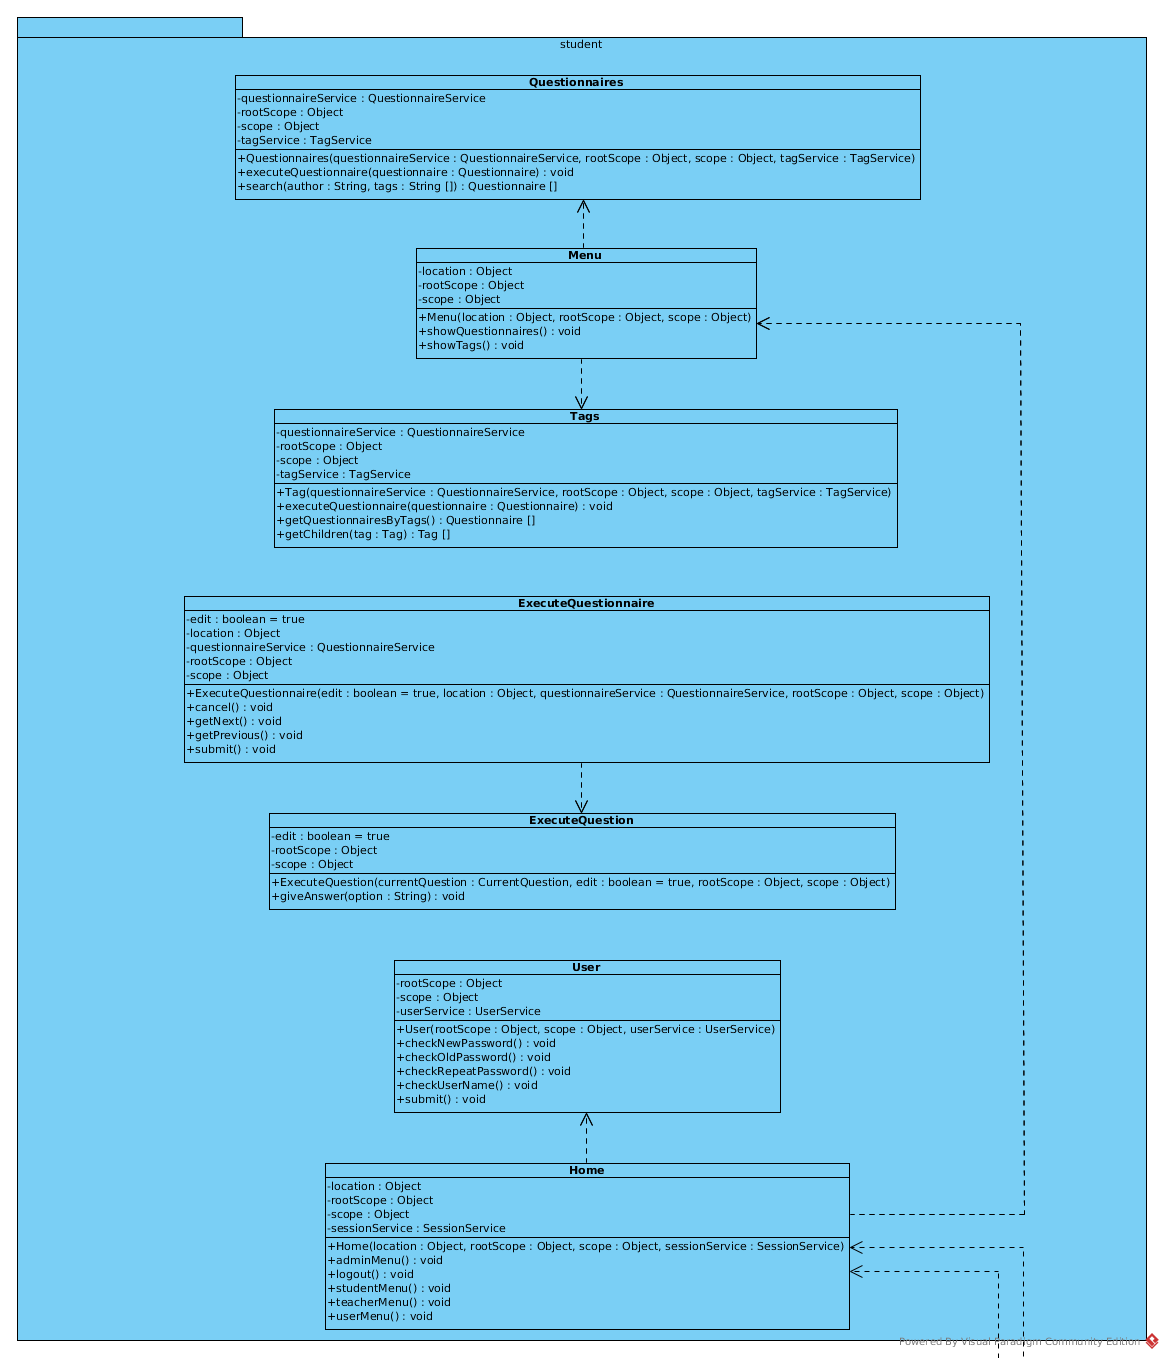
\includegraphics[scale=4, max width=\textwidth, max height=\myheight]{../img/diagrammiClassi/client/controller/student.png}
		\caption{Diagramma package - client::controller::student}
	\end{figure}
\end{center}\hypertarget{client::controller::student::Questionnaires}{}
\subsubsubsection[Questionnaires]{client::controller::student::Questionnaires}
\begin{figure}[H]
	\centering
	\begin{tikzpicture}
	\umlclass{client::controller::student::Questionnaires} {--scope : \$scope\\--questionnaireService : QuestionnaireService\\--tagService : TagService\\--questList : Questionnaire[]\\--userService : UserService\\--titleSearch : String\\--tagSearch : String\\--authorSearch : String\\--myOrderBy : String\\--location : \$location}{+Questionnaires(userService : UserService, questionnaireService : QuestionnaireService, rootScope : Object, scope : Object, tagService : TagService)\\+executeQuestionnaire(questID : integer) : void\\+submit() : void\\+setMyOrderBy(myOrderBy : String) : void\\+setAuthorSearch(authorSearch : String) : void\\+setQuestList(questList : Questionnaire[]) : void\\+setTagSearch(tagSearch : String) : void\\+setTitleSearch(titleSearch : String) : void\\+getAuthorSearch() : String\\+getQuestList() : Questionnaire []\\+getTagSearch() : String\\+getTitleSearch() : String\\+getMyOrderBy() : String}
	\end{tikzpicture}
	\caption{Diagramma classe - client::controller::student::Questionnaires}
\end{figure}\begin{description}
\item[Descrizione] \hfill \\
Classe che si occupa della ricerca di un questionario da parte di uno studente e dell'eventuale gestione di una richiesta di esecuzione di un questionario
\item[Utilizzo] \hfill \\
Si occupa di gestire la ricerca di un questionario e di permettere ad uno studente di navigare tra i questionari presenti nel sistema per sceglierne eventualmente uno da eseguire
\item[Relazioni con altre classi] \hfill \\
\vspace{-7mm}
\begin{description}
	\item[\hyperlink{client::model::data::Questionnaire}{client::model::data::Questionnaire}] \hfill \\
	Relazione uscente, lista di questionari
	\item[\hyperlink{client::model::service::UserService}{client::model::service::UserService}] \hfill \\
	Relazione uscente, campo dati che rappresenta un oggetto UserService
	\item[\hyperlink{client::model::service::TagService}{client::model::service::TagService}] \hfill \\
	Relazione uscente, campo dati che rappresenta un oggetto TagService
	\item[\hyperlink{client::model::service::QuestionnaireService}{client::model::service::QuestionnaireService}] \hfill \\
	Relazione uscente, campo dati che rappresenta un oggetto QuestionnaireService
\end{description}

\item[Attributi] \hfill \\
\vspace{-7mm}
\begin{itemize}
	\item scope : \$scope $\rightarrow$ oggetto di angular che fa riferimento ad una porzione di model di pertinenza di uno specifico controller
	\item questionnaireService : QuestionnaireService $\rightarrow$ campo dati che rappresenta un oggetto QuestionnaireService
	\item tagService : TagService $\rightarrow$ campo dati che rappresenta un oggetto TagService
	\item questList : Questionnaire[] $\rightarrow$ lista di questionari
	\item userService : UserService $\rightarrow$ campo dati che rappresenta un oggetto UserService
	\item titleSearch : String $\rightarrow$ rappresenta il campo titleSearch nella View
	\item tagSearch : String $\rightarrow$ rappresenta il campo tagSearch nella View
	\item authorSearch : String $\rightarrow$ rappresenta il campo authorSearch nella View
	\item myOrderBy : String $\rightarrow$ stringa che si riferisce al campo per cui ordinare i questionari
	\item location : \$location $\rightarrow$ oggetto di angular che analizza l'URL nella barra degli indirizzi del browser e lo rende disponibile all'applicazione
\end{itemize}

\item[Metodi] \hfill \\
\vspace{-7mm}
\begin{itemize}
	\item Questionnaires(userService : UserService, questionnaireService : QuestionnaireService, rootScope : Object, scope : Object, tagService : TagService) $\rightarrow$ costruttore della classe\begin{itemize}
		\item userService $\rightarrow$ campo dati che rappresenta un oggetto UserService
		\item questionnaireService $\rightarrow$ campo dati che rappresenta un oggetto QuestionnaireService
		\item rootScope $\rightarrow$ oggetto di angular che identifica l’elemento con attributo ng-app
		\item scope $\rightarrow$ oggetto di angular che fa riferimento ad una porzione di model di pertinenza di uno specifico controller
		\item tagService $\rightarrow$ campo dati che rappresenta un oggetto TagService 
	\end{itemize}
	
	\item executeQuestionnaire(questID : integer) : void $\rightarrow$ permette di eseguire il questionario passato come parametro caricandone la relativa view\begin{itemize}
		\item questID $\rightarrow$ contiene l'ID del questionario da eseguire
	\end{itemize}
	
	\item submit() : void $\rightarrow$ permette di ricercare questionari filtrandoli in base ad autore, titolo e argomenti, richiamando gli opportuni servizi che mandano la richiesta al server
	\item setMyOrderBy(myOrderBy : String) : void $\rightarrow$ metodo che cambia il valore del campo dati myOrderBy\begin{itemize}
		\item myOrderBy $\rightarrow$ stringa che si riferisce al campo per cui ordinare i questionari
	\end{itemize}
	
	\item setAuthorSearch(authorSearch : String) : void $\rightarrow$ metodo che cambia il valore del campo dati authorSearch\begin{itemize}
		\item authorSearch $\rightarrow$ rappresenta il campo authorSearch nella View
	\end{itemize}
	
	\item setQuestList(questList : Questionnaire[]) : void $\rightarrow$ metodo che cambia il valore del campo dati questList\begin{itemize}
		\item questList $\rightarrow$ lista di questionari
	\end{itemize}
	
	\item setTagSearch(tagSearch : String) : void $\rightarrow$ metodo che cambia il valore del campo dati tagSearch\begin{itemize}
		\item tagSearch $\rightarrow$ rappresenta il campo tagSearch nella View
	\end{itemize}
	
	\item setTitleSearch(titleSearch : String) : void $\rightarrow$ metodo che cambia il valore del campo dati titleSearch\begin{itemize}
		\item titleSearch $\rightarrow$ rappresenta il campo titleSearch nella View
	\end{itemize}
	
	\item getAuthorSearch() : String $\rightarrow$ metodo che restituisce il valore del campo dati authorSearch
	\item getQuestList() : Questionnaire [] $\rightarrow$ metodo che restituisce il valore del campo dati questList
	\item getTagSearch() : String $\rightarrow$ metodo che restituisce il valore del campo dati tagSearch
	\item getTitleSearch() : String $\rightarrow$ metodo che restituisce il valore del campo dati titleSearch
	\item getMyOrderBy() : String $\rightarrow$ metodo che restituisce il valore del campo dati myOrderBy
\end{itemize}

\end{description}

\vspace{0.5cm}
\hypertarget{client::controller::student::ExecuteQuestionnaire}{}
\subsubsubsection[ExecuteQuestionnaire]{client::controller::student::ExecuteQuestionnaire}
\begin{figure}[H]
	\centering
	\begin{tikzpicture}
	\umlclass{client::controller::student::ExecuteQuestionnaire} {--questionnaireService : QuestionnaireService\\--scope : \$scope\\--questionnaire : CurrentQuestionnaire\\--currentQuestion : ExecuteQuestion\\--util : Util\\--q : \$q\\--answerService : AnswerService}{+ExecuteQuestionnaire(location : Object, questionnaireService : QuestionnaireService, rootScope : Object, scope : Object, edit : boolean)\\+getNext() : void\\+getPrevious() : void\\+submit() : void}
	\end{tikzpicture}
	\caption{Diagramma classe - client::controller::student::ExecuteQuestionnaire}
\end{figure}\begin{description}
\item[Descrizione] \hfill \\
La classe che controlla esecuzione del questionario 
\item[Utilizzo] \hfill \\
Viene chiamata quando uno studente comincia a rispondere ad un questionario. Lo studente non è obbligato a rispondere alle domande una dopo l'altra, ha la possibilità di poter tornare su domande che in precedenza non aveva risposto. Solo dopo il submit che il questionario si considera completato
\item[Relazioni con altre classi] \hfill \\
\vspace{-7mm}
\begin{description}
	\item[\hyperlink{client::model::data::CurrentQuestionnaire}{client::model::data::CurrentQuestionnaire}] \hfill \\
	Relazione uscente, istanza del questionario in esecuzione
	\item[\hyperlink{client::controller::student::ExecuteQuestion}{client::controller::student::ExecuteQuestion}] \hfill \\
	Relazione uscente, oggetto controller di ExecuteQuestion che gestisce la domanda corrente
	\item[\hyperlink{client::util::Util}{client::util::Util}] \hfill \\
	Relazione uscente, campo dati che rappresenta un oggetto Util
	\item[\hyperlink{client::model::service::QuestionnaireService}{client::model::service::QuestionnaireService}] \hfill \\
	Relazione uscente, campo dati che rappresenta un oggetto QuestionnaireService
	\item[\hyperlink{client::model::service::AnswerService}{client::model::service::AnswerService}] \hfill \\
	Relazione uscente, campo dati che rappresenta un oggetto AnswerService	
\end{description}

\item[Attributi] \hfill \\
\vspace{-7mm}
\begin{itemize}
	\item questionnaireService : QuestionnaireService $\rightarrow$ campo dati che rappresenta un oggetto QuestionnaireService
	\item scope : \$scope $\rightarrow$ oggetto di angular che fa riferimento ad una porzione di model di pertinenza di uno specifico controller
	\item questionnaire : CurrentQuestionnaire $\rightarrow$ istanza del questionario in esecuzione
	\item currentQuestion : ExecuteQuestion $\rightarrow$ oggetto controller di ExecuteQuestion che gestisce la domanda corrente
	\item util : Util $\rightarrow$ campo dati che rappresenta un oggetto Util
	\item q : \$q $\rightarrow$ oggetto di angular che permette di eseguire funzioni asincrone
	\item answerService : AnswerService $\rightarrow$ campo dati che rappresenta un oggetto AnswerService	
\end{itemize}

\item[Metodi] \hfill \\
\vspace{-7mm}
\begin{itemize}
	\item ExecuteQuestionnaire(location : Object, questionnaireService : QuestionnaireService, rootScope : Object, scope : Object, edit : boolean) $\rightarrow$ costruttore della classe\begin{itemize}
		\item location $\rightarrow$ oggetto di angular che analizza l'URL nella barra degli indirizzi del browser e lo rende disponibile all'applicazione
		\item questionnaireService $\rightarrow$ campo dati che rappresenta un oggetto QuestionnaireService
		\item rootScope $\rightarrow$ oggetto di angular che identifica l’elemento con attributo ng-app
		\item scope $\rightarrow$ oggetto di angular che fa riferimento ad una porzione di model di pertinenza di uno specifico controller
		\item edit $\rightarrow$ indica se esecuzione del questionario è in modalità read-only. Ovvero se variabile è true allora si possono cambiare le risposte alle domande, altrimenti si può solo visualizzare il questionario senza poter cambiare le risposte già selezionate 
	\end{itemize}
	
	\item getNext() : void $\rightarrow$ carica la prossima domanda in executeQuestion
	\item getPrevious() : void $\rightarrow$ carica a domanda precedente in executeQuestion
	\item submit() : void $\rightarrow$ controlla che tutte le risposte siano state date, in caso positivo richiama il metodo per ottenere i risultati e li visualizza, altrimenti visualizza un messaggio di errore
\end{itemize}

\end{description}

\vspace{0.5cm}
\hypertarget{client::controller::student::ExecuteQuestion}{}
\subsubsubsection[ExecuteQuestion]{client::controller::student::ExecuteQuestion}
\begin{figure}[H]
	\centering
	\begin{tikzpicture}
	\umlclass{client::controller::student::ExecuteQuestion} {--scope : \$scope\\--interpolate : \$interpolate\\--sce : \$sce}{+ExecuteQuestion(currentQuestion : CurrentQuestion, edit : boolean, rootScope : Object, scope : Object)\\+giveAnswer(option : String) : void\\+setCurrentQuestion(currentQuestion : currentQuesion) : void}
	\end{tikzpicture}
	\caption{Diagramma classe - client::controller::student::ExecuteQuestion}
\end{figure}\begin{description}
\item[Descrizione] \hfill \\
La classe che controlla l'esecuzione di una domanda 
\item[Utilizzo] \hfill \\
Viene chiamata per dare la possibilità ad uno studente di eseguire una specifica domanda all'interno di un questionario in esecuzione
\item[Relazioni con altre classi] \hfill \\
\vspace{-7mm}
\begin{description}
	\item[\hyperlink{client::controller::student::ExecuteQuestionnaire}{client::controller::student::ExecuteQuestionnaire}] \hfill \\
	Relazione entrante, oggetto controller di ExecuteQuestion che gestisce la domanda corrente
\end{description}

\item[Attributi] \hfill \\
\vspace{-7mm}
\begin{itemize}
	\item scope : \$scope $\rightarrow$ oggetto di angular che fa riferimento ad una porzione di model di pertinenza di uno specifico controller
	\item interpolate : \$interpolate $\rightarrow$ oggetto di angular che permette l'interpolazione di stringhe
	\item sce : \$sce $\rightarrow$ oggetto di angular che permette il trattamento di stringhe in alcuni contesti dove richiedono di essere marcate come sicure
\end{itemize}

\item[Metodi] \hfill \\
\vspace{-7mm}
\begin{itemize}
	\item ExecuteQuestion(currentQuestion : CurrentQuestion, edit : boolean, rootScope : Object, scope : Object) $\rightarrow$ costruttore della classe\begin{itemize}
		\item currentQuestion $\rightarrow$ contiene la domanda corrente da eseguire 
		\item edit $\rightarrow$ true - si può modificare, false - no 
		\item rootScope $\rightarrow$ oggetto di angular che identifica l’elemento con attributo ng-app
		\item scope $\rightarrow$ oggetto di angular che fa riferimento ad una porzione di model di pertinenza di uno specifico controller
	\end{itemize}
	
	\item giveAnswer(option : String) : void $\rightarrow$ metodo che viene chiamato ogni volta che viene modificata la risposta data e la memorizza in currentQuestion\begin{itemize}
		\item option $\rightarrow$ contiene la risposta alla domanda  data dall'utente 
	\end{itemize}
	
	\item setCurrentQuestion(currentQuestion : currentQuesion) : void $\rightarrow$ metodo che cambia la currentQuestion in esecuzione. Questo metodo viene chiamato da executeQuestionnaire quando viene selezionata la domanda successiva o precedente\begin{itemize}
		\item currentQuestion $\rightarrow$ currentQuestion da caricare in esecuzione
	\end{itemize}
	
\end{itemize}

\end{description}

\vspace{0.5cm}
\subsubsection{client::controller::teacher}
È il package che contiene tutte le classi che costituiscono i controller della porzione client per un docente. Ogni componente si occupa della gestione di una particolare porzione dell'interfaccia di un docente.\begin{center}
	\begin{figure}[H]
		\centering 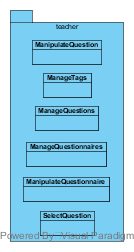
\includegraphics[scale=4, max width=\textwidth, max height=\myheight]{../img/diagrammiClassi/client/controller/teacher.png}
		\caption{Diagramma package - client::controller::teacher}
	\end{figure}
\end{center}\hypertarget{client::controller::teacher::ManipulateQuestion}{}
\subsubsubsection[ManipulateQuestion]{client::controller::teacher::ManipulateQuestion}
\begin{figure}[H]
	\centering
	\begin{tikzpicture}
	\umlclass{client::controller::teacher::ManipulateQuestion} {--question : Question \\--rootScope : \$rootScope\\--questionService : QuestionService\\--scope : \$scope\\--tagService : TagService\\--location : \$location\\--qml : QML\\--error : Error\\--edit : boolean\\--editor : SimpleMDE\\--tagsInput : String\\--tags : Tag []\\--editorBuilder : Editor}{+ManipulateQuestion(question : Question, questionService : QuestionService, scope : Object, rootScope : Object)\\+submit() : void\\+getError() : Error\\+setError(error : Error) : void\\+getEditor() : SimpleMDE\\+getEdit() : boolean\\+getQuestion() : Question \\+getTags() : Tag []\\+getTagsInput() : String\\+setEditor(editor : SimpleMDE) : void\\+setEdit(edit : boolean) : void\\+setQuestion(question : Question ) : void\\+setTags(tags : Tag []) : void\\+setTagsInput(tagsInput : String) : void}
	\end{tikzpicture}
	\caption{Diagramma classe - client::controller::teacher::ManipulateQuestion}
\end{figure}\begin{description}
\item[Descrizione] \hfill \\
Classe che si occupa della gestione della domanda lato docente
\item[Utilizzo] \hfill \\
Viene richiamata quando un docente vuole aggiungere,  modificare o eliminare una domanda
\item[Relazioni con altre classi] \hfill \\
\vspace{-7mm}
\begin{description}
	\item[\hyperlink{client::model::data::Question}{client::model::data::Question}] \hfill \\
	Relazione uscente, oggetto che rappresenta una singola domanda
	\item[\hyperlink{client::model::service::TagService}{client::model::service::TagService}] \hfill \\
	Relazione uscente, campo dati che rappresenta un oggetto TagService
	\item[\hyperlink{client::util::QML}{client::util::QML}] \hfill \\
	Relazione uscente, campo dati che rappresenta un oggetto QML
	\item[\hyperlink{client::model::data::Error}{client::model::data::Error}] \hfill \\
	Relazione uscente, campo dati che rappresenta un oggetto Error
	\item[\hyperlink{client::model::data::Tag}{client::model::data::Tag}] \hfill \\
	Relazione uscente, argomenti che compaiono nei suggerimenti
	\item[\hyperlink{client::model::service::QuestionService}{client::model::service::QuestionService}] \hfill \\
	Relazione uscente, campo dati che rappresenta un oggetto QuestionService
	\item[\hyperlink{client::util::Editor}{client::util::Editor}] \hfill \\
	Relazione uscente, campo dati che rappresenta un oggetto Editor
\end{description}

\item[Attributi] \hfill \\
\vspace{-7mm}
\begin{itemize}
	\item question : Question  $\rightarrow$ oggetto che rappresenta una singola domanda
	\item rootScope : \$rootScope $\rightarrow$ oggetto di angular che identifica l’elemento con attributo ng-app
	\item questionService : QuestionService $\rightarrow$ campo dati che rappresenta un oggetto QuestionService
	\item scope : \$scope $\rightarrow$ oggetto di angular che fa riferimento ad una porzione di model di pertinenza di uno specifico controller
	\item tagService : TagService $\rightarrow$ campo dati che rappresenta un oggetto TagService
	\item location : \$location $\rightarrow$ oggetto di angular che analizza l'URL nella barra degli indirizzi del browser e lo rende disponibile all'applicazione
	\item qml : QML $\rightarrow$ campo dati che rappresenta un oggetto QML
	\item error : Error $\rightarrow$ campo dati che rappresenta un oggetto Error
	\item edit : boolean $\rightarrow$ indica se la domanda corrente è nuova o se si sta modificando una già creata
	\item editor : SimpleMDE $\rightarrow$ oggetto che rappreseta l'editor per manipolare la domanda
	\item tagsInput : String $\rightarrow$ rappresenta il campo tagsInput nella View
	\item tags : Tag [] $\rightarrow$ argomenti che compaiono nei suggerimenti
	\item editorBuilder : Editor $\rightarrow$ campo dati che rappresenta un oggetto Editor
\end{itemize}

\item[Metodi] \hfill \\
\vspace{-7mm}
\begin{itemize}
	\item ManipulateQuestion(question : Question, questionService : QuestionService, scope : Object, rootScope : Object) $\rightarrow$ costruttore della classe\begin{itemize}
		\item question $\rightarrow$ contiene il riferimento verso il modello delle domande 
		\item questionService $\rightarrow$ campo dati che rappresenta un oggetto QuestionService
		\item scope $\rightarrow$ oggetto di angular che fa riferimento ad una porzione di model di pertinenza di uno specifico controller
		\item rootScope $\rightarrow$ oggetto di angular che identifica l’elemento con attributo ng-app
	\end{itemize}
	
	\item submit() : void $\rightarrow$ dopo aver controllato la validità del titolo, tags e QML inseriti, invia i dati al servizio che si occupa di inserire la domanda nel sistema
	\item getError() : Error $\rightarrow$ metodo che restituisce il valore del campo dati error
	\item setError(error : Error) : void $\rightarrow$ metodo che cambia il valore del campo dati error\begin{itemize}
		\item error $\rightarrow$ campo dati che rappresenta un oggetto Error
	\end{itemize}
	
	\item getEditor() : SimpleMDE $\rightarrow$ metodo che restituisce il valore del campo dati editor
	\item getEdit() : boolean $\rightarrow$ metodo che restituisce il valore del campo dati edit
	\item getQuestion() : Question  $\rightarrow$ metodo che restituisce il valore del campo dati question
	\item getTags() : Tag [] $\rightarrow$ metodo che restituisce il valore del campo dati tags
	\item getTagsInput() : String $\rightarrow$ metodo che restituisce il valore del campo dati tagsInput
	\item setEditor(editor : SimpleMDE) : void $\rightarrow$ metodo che cambia il valore del campo dati editor\begin{itemize}
		\item editor $\rightarrow$ oggetto che rappreseta l'editor per manipolare la domanda
	\end{itemize}
	
	\item setEdit(edit : boolean) : void $\rightarrow$ metodo che cambia il valore del campo dati edit\begin{itemize}
		\item edit $\rightarrow$ indica se la domanda corrente è nuova o se si sta modificando una già creata
	\end{itemize}
	
	\item setQuestion(question : Question ) : void $\rightarrow$ metodo che cambia il valore del campo dati question\begin{itemize}
		\item question $\rightarrow$ oggetto che rappresenta una singola domanda
	\end{itemize}
	
	\item setTags(tags : Tag []) : void $\rightarrow$ metodo che cambia il valore del campo dati tags\begin{itemize}
		\item tags $\rightarrow$ argomenti che compaiono nei suggerimenti
	\end{itemize}
	
	\item setTagsInput(tagsInput : String) : void $\rightarrow$ metodo che cambia il valore del campo dati tagsInput\begin{itemize}
		\item tagsInput $\rightarrow$ rappresenta il campo tagsInput nella View
	\end{itemize}
	
\end{itemize}

\end{description}

\vspace{0.5cm}
\hypertarget{client::controller::teacher::ManipulateQuestionnaire}{}
\subsubsubsection[ManipulateQuestionnaire]{client::controller::teacher::ManipulateQuestionnaire}
\begin{figure}[H]
	\centering
	\begin{tikzpicture}
	\umlclass{client::controller::teacher::ManipulateQuestionnaire} {--questionnaire : Questionnaire\\--questionnaireService : QuestionnaireService\\--rootScope : \$rootScope\\--scope : \$scope\\--edit : boolean\\--location : \$location\\--qml : QML\\--questionService : QuestionService\\--tagService : TagService\\--userService : UserService\\--error : Error\\--onSelect : boolean\\--tagsInput : String\\--tags : Tag []}{+ManipulateQuestionnaire(questionnaireService : QuestionnaireService, questionnaire : Questionnaire, scope : Object, rootScope : Object)\\+addQuestion(question : Question) : void\\+removeQuestion(question : Question) : void\\+submit() : void\\+preview() : void\\+getError() : Error\\+setError(error : Error) : void\\+getEdit() : boolean\\+getOnSelect() : boolean\\+getQuestionnaire() : Questionnaire\\+getTags() : Tag []\\+getTagsInput() : String\\+setEdit(edit : boolean) : void\\+setOnSelect(onSelect : boolean) : void\\+setQuestionnaire(questionnaire : Questionnaire) : void\\+setTags(tags : Tag []) : void\\+setTagsInput(tagsInput : String) : void}
	\end{tikzpicture}
	\caption{Diagramma classe - client::controller::teacher::ManipulateQuestionnaire}
\end{figure}\begin{description}
\item[Descrizione] \hfill \\
Classe che si occupa della gestione di un questionario lato docente
\item[Utilizzo] \hfill \\
Viene richiamata quando un docente vuole creare un nuovo questionario o modificare o eliminare uno già esistente
\item[Relazioni con altre classi] \hfill \\
\vspace{-7mm}
\begin{description}
	\item[\hyperlink{client::model::data::Questionnaire}{client::model::data::Questionnaire}] \hfill \\
	Relazione uscente, oggetto che rappresenta un questionario
	\item[\hyperlink{client::util::QML}{client::util::QML}] \hfill \\
	Relazione uscente, campo dati che rappresenta un oggetto QML
	\item[\hyperlink{client::model::service::QuestionService}{client::model::service::QuestionService}] \hfill \\
	Relazione uscente, campo dati che rappresenta un oggetto QuestionService
	\item[\hyperlink{client::model::service::TagService}{client::model::service::TagService}] \hfill \\
	Relazione uscente, campo dati che rappresenta un oggetto TagService
	\item[\hyperlink{client::model::service::UserService}{client::model::service::UserService}] \hfill \\
	Relazione uscente, campo dati che rappresenta un oggetto UserService
	\item[\hyperlink{client::model::data::Error}{client::model::data::Error}] \hfill \\
	Relazione uscente, campo dati che rappresenta un oggetto Error
	\item[\hyperlink{client::model::data::Tag}{client::model::data::Tag}] \hfill \\
	Relazione uscente, argomenti che compaiono nei suggerimenti
	\item[\hyperlink{client::model::service::QuestionnaireService}{client::model::service::QuestionnaireService}] \hfill \\
	Relazione uscente, campo dati che rappresenta un oggetto QuestionnaireService
\end{description}

\item[Attributi] \hfill \\
\vspace{-7mm}
\begin{itemize}
	\item questionnaire : Questionnaire $\rightarrow$ oggetto che rappresenta un questionario
	\item questionnaireService : QuestionnaireService $\rightarrow$ campo dati che rappresenta un oggetto QuestionnaireService
	\item rootScope : \$rootScope $\rightarrow$ oggetto di angular che identifica l’elemento con attributo ng-app
	\item scope : \$scope $\rightarrow$ oggetto di angular che fa riferimento ad una porzione di model di pertinenza di uno specifico controller
	\item edit : boolean $\rightarrow$ indica se il questionario corrente è nuovo o se si sta modificando uno già creato
	\item location : \$location $\rightarrow$ oggetto di angular che analizza l'URL nella barra degli indirizzi del browser e lo rende disponibile all'applicazione
	\item qml : QML $\rightarrow$ campo dati che rappresenta un oggetto QML
	\item questionService : QuestionService $\rightarrow$ campo dati che rappresenta un oggetto QuestionService
	\item tagService : TagService $\rightarrow$ campo dati che rappresenta un oggetto TagService
	\item userService : UserService $\rightarrow$ campo dati che rappresenta un oggetto UserService
	\item error : Error $\rightarrow$ campo dati che rappresenta un oggetto Error
	\item onSelect : boolean $\rightarrow$ indica se si è in fase di selezione di una domanda da aggiungere
	\item tagsInput : String $\rightarrow$ rappresenta il campo tagsInput nella View
	\item tags : Tag [] $\rightarrow$ argomenti che compaiono nei suggerimenti
\end{itemize}

\item[Metodi] \hfill \\
\vspace{-7mm}
\begin{itemize}
	\item ManipulateQuestionnaire(questionnaireService : QuestionnaireService, questionnaire : Questionnaire, scope : Object, rootScope : Object) $\rightarrow$ costruttore della classe\begin{itemize}
		\item questionnaireService $\rightarrow$ campo dati che rappresenta un oggetto QuestionnaireService
		\item questionnaire $\rightarrow$ contiene il riferimento al modello degli questionari 
		\item scope $\rightarrow$ oggetto di angular che fa riferimento ad una porzione di model di pertinenza di uno specifico controller
		\item rootScope $\rightarrow$ oggetto di angular che identifica l’elemento con attributo ng-app
	\end{itemize}
	
	\item addQuestion(question : Question) : void $\rightarrow$ aggiunge la domanda passata come parametro al questionario d'istanza\begin{itemize}
		\item question $\rightarrow$ contiene la domanda da aggiungere al questionario 
	\end{itemize}
	
	\item removeQuestion(question : Question) : void $\rightarrow$ rimuove la domanda passata per parametro dal questionario d'istanza\begin{itemize}
		\item question $\rightarrow$ contiene la domanda da eliminare dal questionario 
	\end{itemize}
	
	\item submit() : void $\rightarrow$ dopo aver controllato la validità delle domande, titolo e tags inseriti, invia i dati presenti nel questionario al servizio che si occupa di aggiungerlo al sistema
	\item preview() : void $\rightarrow$ provvede a fornire un'anteprima di una domanda da QML in HTML
	\item getError() : Error $\rightarrow$ metodo che restituisce il valore del campo dati error
	\item setError(error : Error) : void $\rightarrow$ metodo che cambia il valore del campo dati error\begin{itemize}
		\item error $\rightarrow$ campo dati che rappresenta un oggetto Error
	\end{itemize}
	
	\item getEdit() : boolean $\rightarrow$ metodo che restituisce il valore del campo dati edit
	\item getOnSelect() : boolean $\rightarrow$ metodo che restituisce il valore del campo dati onSelect
	\item getQuestionnaire() : Questionnaire $\rightarrow$ metodo che restituisce il valore del campo dati questionnaire
	\item getTags() : Tag [] $\rightarrow$ metodo che restituisce il valore del campo dati tags
	\item getTagsInput() : String $\rightarrow$ metodo che restituisce il valore del campo dati tagsInput
	\item setEdit(edit : boolean) : void $\rightarrow$ metodo che cambia il valore del campo dati edit\begin{itemize}
		\item edit $\rightarrow$ indica se il questionario corrente è nuovo o se si sta modificando uno già creato
	\end{itemize}
	
	\item setOnSelect(onSelect : boolean) : void $\rightarrow$ metodo che cambia il valore del campo dati onSelect\begin{itemize}
		\item onSelect $\rightarrow$ indica se si è in fase di selezione di una domanda da aggiungere
	\end{itemize}
	
	\item setQuestionnaire(questionnaire : Questionnaire) : void $\rightarrow$ metodo che cambia il valore del campo dati questionnaire\begin{itemize}
		\item questionnaire $\rightarrow$ oggetto che rappresenta un questionario
	\end{itemize}
	
	\item setTags(tags : Tag []) : void $\rightarrow$ metodo che cambia il valore del campo dati tags\begin{itemize}
		\item tags $\rightarrow$ argomenti che compaiono nei suggerimenti
	\end{itemize}
	
	\item setTagsInput(tagsInput : String) : void $\rightarrow$ metodo che cambia il valore del campo dati tagsInput\begin{itemize}
		\item tagsInput $\rightarrow$ rappresenta il campo tagsInput nella View
	\end{itemize}
	
\end{itemize}

\end{description}

\vspace{0.5cm}
\hypertarget{client::controller::teacher::SelectQuestion}{}
\subsubsubsection[SelectQuestion]{client::controller::teacher::SelectQuestion}
\begin{figure}[H]
	\centering
	\begin{tikzpicture}
	\umlclass{client::controller::teacher::SelectQuestion} {--questionService : QuestionService\\--scope : \$scope\\--tagService : TagService\\--userService : UserService\\--q : \$q\\--authorSearch : String\\--tagSearch : String\\--bodySearch : String\\--questions : Question []}{+SelectQuestion(questionService : QuestionService, rootScope : Object, scope : Object)\\+submit(author : String, keywordsQuery : String) : void\\+getAuthorSearch() : String\\+getBodySearch() : String\\+getQuestions() : Question []\\+getTagSearch() : String\\+setAuthorSearch(authorSearch : String) : void\\+setBodySearch(bodySearch : String) : void\\+setQuestions(questions : Question []) : void\\+setTagSearch(tagSearch : String) : void}
	\end{tikzpicture}
	\caption{Diagramma classe - client::controller::teacher::SelectQuestion}
\end{figure}\begin{description}
\item[Descrizione] \hfill \\
Classe che gestisce la ricerca di una domanda e la sua eventuale selezione
\item[Utilizzo] \hfill \\
Viene chiamata quando in fase di costruzione di un questionario si ha la necessità di ricercare per poi inserire una particolare domanda
\item[Relazioni con altre classi] \hfill \\
\vspace{-7mm}
\begin{description}
	\item[\hyperlink{client::model::service::TagService}{client::model::service::TagService}] \hfill \\
	Relazione uscente, campo dati che rappresenta un oggetto TagService
	\item[\hyperlink{client::model::service::UserService}{client::model::service::UserService}] \hfill \\
	Relazione uscente, campo dati che rappresenta un oggetto UserService
	\item[\hyperlink{client::model::data::Question}{client::model::data::Question}] \hfill \\
	Relazione uscente, domande visualizzate nella view
	\item[\hyperlink{client::model::service::QuestionService}{client::model::service::QuestionService}] \hfill \\
	Relazione uscente, campo dati che rappresenta un oggetto QuestionService
\end{description}

\item[Attributi] \hfill \\
\vspace{-7mm}
\begin{itemize}
	\item questionService : QuestionService $\rightarrow$ campo dati che rappresenta un oggetto QuestionService
	\item scope : \$scope $\rightarrow$ oggetto di angular che fa riferimento ad una porzione di model di pertinenza di uno specifico controller
	\item tagService : TagService $\rightarrow$ campo dati che rappresenta un oggetto TagService
	\item userService : UserService $\rightarrow$ campo dati che rappresenta un oggetto UserService
	\item q : \$q $\rightarrow$ oggetto di angular che permette di eseguire funzioni asincrone
	\item authorSearch : String $\rightarrow$ rappresenta il campo authorSearch nella View
	\item tagSearch : String $\rightarrow$ rappresenta il campo tagSearch nella View
	\item bodySearch : String $\rightarrow$ rappresenta il campo bodySearch nella View
	\item questions : Question [] $\rightarrow$ domande visualizzate nella view
\end{itemize}

\item[Metodi] \hfill \\
\vspace{-7mm}
\begin{itemize}
	\item SelectQuestion(questionService : QuestionService, rootScope : Object, scope : Object) $\rightarrow$ costruttore della classe\begin{itemize}
		\item questionService $\rightarrow$ campo dati che rappresenta un oggetto QuestionService
		\item rootScope $\rightarrow$ oggetto di angular che identifica l’elemento con attributo ng-app
		\item scope $\rightarrow$ oggetto di angular che fa riferimento ad una porzione di model di pertinenza di uno specifico controller
	\end{itemize}
	
	\item submit(author : String, keywordsQuery : String) : void $\rightarrow$ trova tutte le domande correlate ad un autore e a delle parole chiave passati come parametro\begin{itemize}
		\item author $\rightarrow$ contiene il nome dell'autore della domanda da ricercare 
		\item keywordsQuery $\rightarrow$ contiene la lista di parole chiave per ricercare la domanda
	\end{itemize}
	
	\item getAuthorSearch() : String $\rightarrow$ metodo che restituisce il valore del campo dati authorSearch
	\item getBodySearch() : String $\rightarrow$ metodo che restituisce il valore del campo dati bodySearch
	\item getQuestions() : Question [] $\rightarrow$ metodo che restituisce il valore del campo dati questions
	\item getTagSearch() : String $\rightarrow$ metodo che restituisce il valore del campo dati tagSearch
	\item setAuthorSearch(authorSearch : String) : void $\rightarrow$ metodo che cambia il valore del campo dati authorSearch\begin{itemize}
		\item authorSearch $\rightarrow$ rappresenta il campo authorSearch nella View
	\end{itemize}
	
	\item setBodySearch(bodySearch : String) : void $\rightarrow$ metodo che cambia il valore del campo dati bodySearch\begin{itemize}
		\item bodySearch $\rightarrow$ rappresenta il campo bodySearch nella View
	\end{itemize}
	
	\item setQuestions(questions : Question []) : void $\rightarrow$ metodo che cambia il valore del campo dati questions\begin{itemize}
		\item questions $\rightarrow$ domande visualizzate nella view
	\end{itemize}
	
	\item setTagSearch(tagSearch : String) : void $\rightarrow$ metodo che cambia il valore del campo dati tagSearch\begin{itemize}
		\item tagSearch $\rightarrow$ rappresenta il campo tagSearch nella View
	\end{itemize}
	
\end{itemize}

\end{description}

\vspace{0.5cm}
\hypertarget{client::controller::teacher::ManageTags}{}
\subsubsubsection[ManageTags]{client::controller::teacher::ManageTags}
\begin{figure}[H]
	\centering
	\begin{tikzpicture}
	\umlclass{client::controller::teacher::ManageTags} {--scope : \$scope\\--tagService : TagService\\--util : Util\\--tagSearch : String\\--newName : String\\--newDescription : String\\--tags : Tag []}{+ManageTags(rootScope : Object, scope : Object, tagService : TagService)\\+add() : void\\+modify(tag : Tag) : void\\+remove (tag : Tag) : void\\+submit() : void\\+getNewDescription() : String\\+getNewName() : String\\+getTags() : Tag []\\+getTagSearch() : String\\+setNewDescription(newDescription : String) : void\\+setNewName(newName : String) : void\\+setTags(tags : Tag []) : void\\+setTagSearch(tagSearch : String) : void}
	\end{tikzpicture}
	\caption{Diagramma classe - client::controller::teacher::ManageTags}
\end{figure}\begin{description}
\item[Descrizione] \hfill \\
Classe che si occupa della gestione degli argomenti lato docente
\item[Utilizzo] \hfill \\
Viene richiamata quando un docente vuole creare un nuovo argomento o modificarne o eliminarne uno già esistente
\item[Relazioni con altre classi] \hfill \\
\vspace{-7mm}
\begin{description}
	\item[\hyperlink{client::util::Util}{client::util::Util}] \hfill \\
	Relazione uscente, campo dati che rappresenta un oggetto Util
	\item[\hyperlink{client::model::data::Tag}{client::model::data::Tag}] \hfill \\
	Relazione uscente, tags visualizzati nella view
	\item[\hyperlink{client::model::service::TagService}{client::model::service::TagService}] \hfill \\
	Relazione uscente, campo dati che rappresenta un oggetto TagService
\end{description}

\item[Attributi] \hfill \\
\vspace{-7mm}
\begin{itemize}
	\item scope : \$scope $\rightarrow$ oggetto di angular che fa riferimento ad una porzione di model di pertinenza di uno specifico controller
	\item tagService : TagService $\rightarrow$ campo dati che rappresenta un oggetto TagService
	\item util : Util $\rightarrow$ campo dati che rappresenta un oggetto Util
	\item tagSearch : String $\rightarrow$ rappresenta il campo tagSearch nella view
	\item newName : String $\rightarrow$ rappresenta il campo newName nella View
	\item newDescription : String $\rightarrow$ rappresenta il campo newDescription nella View
	\item tags : Tag [] $\rightarrow$ tags visualizzati nella view
\end{itemize}

\item[Metodi] \hfill \\
\vspace{-7mm}
\begin{itemize}
	\item ManageTags(rootScope : Object, scope : Object, tagService : TagService) $\rightarrow$ costruttore della classe\begin{itemize}
		\item rootScope $\rightarrow$ oggetto di angular che identifica l’elemento con attributo ng-app
		\item scope $\rightarrow$ oggetto di angular che fa riferimento ad una porzione di model di pertinenza di uno specifico controller
		\item tagService $\rightarrow$ campo dati che rappresenta un oggetto TagService 
	\end{itemize}
	
	\item add() : void $\rightarrow$ dopo aver controllato la validità dei dati inseriti, richiama il servizio per aggiungere un nuovo argomento
	\item modify(tag : Tag) : void $\rightarrow$ richiama il servizio che modifica l'argomento passato come parametro\begin{itemize}
		\item tag $\rightarrow$ contiene l'argomento che serve modificare 
	\end{itemize}
	
	\item remove (tag : Tag) : void $\rightarrow$ richiama il servizio per rimuovere l'argomento passato come parametro\begin{itemize}
		\item tag $\rightarrow$ contiene l'argomento da eliminare 
	\end{itemize}
	
	\item submit() : void $\rightarrow$ cerca i tag filtrandoli in base alle keywords inserite dall'utente
	\item getNewDescription() : String $\rightarrow$ metodo che restituisce il valore del campo dati newDescription
	\item getNewName() : String $\rightarrow$ metodo che restituisce il valore del campo dati newName
	\item getTags() : Tag [] $\rightarrow$ metodo che restituisce il valore del campo dati tags
	\item getTagSearch() : String $\rightarrow$ metodo che restituisce il valore del campo dati tagSearch
	\item setNewDescription(newDescription : String) : void $\rightarrow$ metodo che cambia il valore del campo dati newDescription\begin{itemize}
		\item newDescription $\rightarrow$ rappresenta il campo newDescription nella View
	\end{itemize}
	
	\item setNewName(newName : String) : void $\rightarrow$ metodo che cambia il valore del campo dati newName\begin{itemize}
		\item newName $\rightarrow$ rappresenta il campo newName nella View
	\end{itemize}
	
	\item setTags(tags : Tag []) : void $\rightarrow$ metodo che cambia il valore del campo dati tags\begin{itemize}
		\item tags $\rightarrow$ tags visualizzati nella view
	\end{itemize}
	
	\item setTagSearch(tagSearch : String) : void $\rightarrow$ metodo che cambia il valore del campo dati tagSearch\begin{itemize}
		\item tagSearch $\rightarrow$ rappresenta il campo tagSearch nella view
	\end{itemize}
	
\end{itemize}

\end{description}

\vspace{0.5cm}
\hypertarget{client::controller::teacher::ManageQuestions}{}
\subsubsubsection[ManageQuestions]{client::controller::teacher::ManageQuestions}
\begin{figure}[H]
	\centering
	\begin{tikzpicture}
	\umlclass{client::controller::teacher::ManageQuestions} {--scope : \$scope\\--rootScope : \$rootScope\\--questionService : QuestionService\\--location : \$location\\--util : Util\\--qml : QML\\--tagService : TagService\\--questions : Question []}{+ManageQuestions(questionnaireService : QuestionnaireService, scope : Object, rootScope : Object)\\+modify(question : Question) : void\\+remove (question : Question) : void\\+preview() : String\\+getQuestions() : Question []\\+setQuestions(questions : Question []) : void}
	\end{tikzpicture}
	\caption{Diagramma classe - client::controller::teacher::ManageQuestions}
\end{figure}\begin{description}
\item[Descrizione] \hfill \\
La classe che controlla la gestione delle domande create dal docente autenticato
\item[Utilizzo] \hfill \\
Viene richiamata quando un docente vuole creare un nuova domanda o modificarne o eliminarne una già esistente tra quelle da lui create
\item[Relazioni con altre classi] \hfill \\
\vspace{-7mm}
\begin{description}
	\item[\hyperlink{client::util::Util}{client::util::Util}] \hfill \\
	Relazione uscente, campo dati che rappresenta un oggetto Util
	\item[\hyperlink{client::util::QML}{client::util::QML}] \hfill \\
	Relazione uscente, campo dati che rappresenta un oggetto QML
	\item[\hyperlink{client::model::service::TagService}{client::model::service::TagService}] \hfill \\
	Relazione uscente, campo dati che rappresenta un oggetto TagService
	\item[\hyperlink{client::model::data::Question}{client::model::data::Question}] \hfill \\
	Relazione uscente, domande visualizzate nella view
	\item[\hyperlink{client::model::service::QuestionService}{client::model::service::QuestionService}] \hfill \\
	Relazione uscente, campo dati che rappresenta un oggetto QuestionService
\end{description}

\item[Attributi] \hfill \\
\vspace{-7mm}
\begin{itemize}
	\item scope : \$scope $\rightarrow$ oggetto di angular che fa riferimento ad una porzione di model di pertinenza di uno specifico controller
	\item rootScope : \$rootScope $\rightarrow$ oggetto di angular che identifica l’elemento con attributo ng-app
	\item questionService : QuestionService $\rightarrow$ campo dati che rappresenta un oggetto QuestionService
	\item location : \$location $\rightarrow$ oggetto di angular che analizza l'URL nella barra degli indirizzi del browser e lo rende disponibile all'applicazione
	\item util : Util $\rightarrow$ campo dati che rappresenta un oggetto Util
	\item qml : QML $\rightarrow$ campo dati che rappresenta un oggetto QML
	\item tagService : TagService $\rightarrow$ campo dati che rappresenta un oggetto TagService
	\item questions : Question [] $\rightarrow$ domande visualizzate nella view
\end{itemize}

\item[Metodi] \hfill \\
\vspace{-7mm}
\begin{itemize}
	\item ManageQuestions(questionnaireService : QuestionnaireService, scope : Object, rootScope : Object) $\rightarrow$ costruttore della classe\begin{itemize}
		\item questionnaireService $\rightarrow$ campo dati che rappresenta un oggetto QuestionnaireService
		\item scope $\rightarrow$ oggetto di angular che fa riferimento ad una porzione di model di pertinenza di uno specifico controller
		\item rootScope $\rightarrow$ oggetto di angular che identifica l’elemento con attributo ng-app
	\end{itemize}
	
	\item modify(question : Question) : void $\rightarrow$ modifica la domanda passata per parametro\begin{itemize}
		\item question $\rightarrow$ contiene  la domanda da modificare 
	\end{itemize}
	
	\item remove (question : Question) : void $\rightarrow$ elimina la domanda passata per parametro\begin{itemize}
		\item question $\rightarrow$ contiene la domanda da eliminare 
	\end{itemize}
	
	\item preview() : String $\rightarrow$ provvede a fornire un'anteprima di una domanda da QML in HTML
	\item getQuestions() : Question [] $\rightarrow$ metodo che restituisce il valore del campo dati questions
	\item setQuestions(questions : Question []) : void $\rightarrow$ metodo che cambia il valore del campo dati questions\begin{itemize}
		\item questions $\rightarrow$ domande visualizzate nella view
	\end{itemize}
	
\end{itemize}

\end{description}

\vspace{0.5cm}
\hypertarget{client::controller::teacher::ManageQuestionnaires}{}
\subsubsubsection[ManageQuestionnaires]{client::controller::teacher::ManageQuestionnaires}
\begin{figure}[H]
	\centering
	\begin{tikzpicture}
	\umlclass{client::controller::teacher::ManageQuestionnaires} {--scope : \$scope\\--rootScope : \$rootScope\\--questionnaireService : QuestionnaireService\\--tagService : TagService\\--location : \$location\\--qml : QML\\--util : Util\\--questionnaires : Questionnaire []}{+ManageQuestionnaires(questionnaireService : QuestionnaireService, scope : Object, rootScope : Object)\\+modify(questionnaire : Questionnaire) : void\\+remove (questionnaire : Questionnaire) : void\\+preview() : String\\+getQuestionnaires() : Questionnaire []\\+setQuestionnaires(questionnaires : Questionnaire []) : void}
	\end{tikzpicture}
	\caption{Diagramma classe - client::controller::teacher::ManageQuestionnaires}
\end{figure}\begin{description}
\item[Descrizione] \hfill \\
La classe che controlla la gestione dei questionari creati dal docente autenticato
\item[Utilizzo] \hfill \\
Viene richiamata quando un docente vuole creare un nuovo questionario o modificarne o eliminarne uno già esistente tra quelli da lui crearti
\item[Relazioni con altre classi] \hfill \\
\vspace{-7mm}
\begin{description}
	\item[\hyperlink{client::model::service::TagService}{client::model::service::TagService}] \hfill \\
	Relazione uscente, campo dati che rappresenta un oggetto TagService
	\item[\hyperlink{client::util::QML}{client::util::QML}] \hfill \\
	Relazione uscente, campo dati che rappresenta un oggetto QML
	\item[\hyperlink{client::util::Util}{client::util::Util}] \hfill \\
	Relazione uscente, campo dati che rappresenta un oggetto Util
	\item[\hyperlink{client::model::data::Questionnaire}{client::model::data::Questionnaire}] \hfill \\
	Relazione uscente, questionari visualizzati nella view
	\item[\hyperlink{client::model::service::QuestionnaireService}{client::model::service::QuestionnaireService}] \hfill \\
	Relazione uscente, campo dati che rappresenta un oggetto QuestionnaireService
\end{description}

\item[Attributi] \hfill \\
\vspace{-7mm}
\begin{itemize}
	\item scope : \$scope $\rightarrow$ oggetto di angular che fa riferimento ad una porzione di model di pertinenza di uno specifico controller
	\item rootScope : \$rootScope $\rightarrow$ oggetto di angular che identifica l’elemento con attributo ng-app
	\item questionnaireService : QuestionnaireService $\rightarrow$ campo dati che rappresenta un oggetto QuestionnaireService
	\item tagService : TagService $\rightarrow$ campo dati che rappresenta un oggetto TagService
	\item location : \$location $\rightarrow$ oggetto di angular che analizza l'URL nella barra degli indirizzi del browser e lo rende disponibile all'applicazione
	\item qml : QML $\rightarrow$ campo dati che rappresenta un oggetto QML
	\item util : Util $\rightarrow$ campo dati che rappresenta un oggetto Util
	\item questionnaires : Questionnaire [] $\rightarrow$ questionari visualizzati nella view
\end{itemize}

\item[Metodi] \hfill \\
\vspace{-7mm}
\begin{itemize}
	\item ManageQuestionnaires(questionnaireService : QuestionnaireService, scope : Object, rootScope : Object) $\rightarrow$ costruttore della classe\begin{itemize}
		\item questionnaireService $\rightarrow$ campo dati che rappresenta un oggetto QuestionnaireService
		\item scope $\rightarrow$ oggetto di angular che fa riferimento ad una porzione di model di pertinenza di uno specifico controller
		\item rootScope $\rightarrow$ oggetto di angular che identifica l’elemento con attributo ng-app
	\end{itemize}
	
	\item modify(questionnaire : Questionnaire) : void $\rightarrow$ modifica il questionario passato come parametro\begin{itemize}
		\item questionnaire $\rightarrow$ contiene il questionario da modificare 
	\end{itemize}
	
	\item remove (questionnaire : Questionnaire) : void $\rightarrow$ elimina il questionario passato come parametro\begin{itemize}
		\item questionnaire $\rightarrow$  Contiene il questionario da eliminare 
	\end{itemize}
	
	\item preview() : String $\rightarrow$ provvede a fornire un'anteprima di una domanda da QML in HTML
	\item getQuestionnaires() : Questionnaire [] $\rightarrow$ metodo che restituisce il valore del campo dati questionnaires
	\item setQuestionnaires(questionnaires : Questionnaire []) : void $\rightarrow$ metodo che cambia il valore del campo dati questionnaires\begin{itemize}
		\item questionnaires $\rightarrow$ questionari visualizzati nella view
	\end{itemize}
	
\end{itemize}

\end{description}

\vspace{0.5cm}
\subsubsection{client::controller::admin}
È il package che contiene tutte le classi che costituiscono i controller della porzione client per un amministratore. Ogni componente si occupa della gestione di una particolare porzione dell'interfaccia di un amministratore.\begin{center}
	\begin{figure}[H]
		\centering 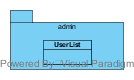
\includegraphics[scale=4, max width=\textwidth, max height=\myheight]{../img/diagrammiClassi/client/controller/admin.png}
		\caption{Diagramma package - client::controller::admin}
	\end{figure}
\end{center}\hypertarget{client::controller::admin::UsersList}{}
\subsubsubsection[UsersList]{client::controller::admin::UsersList}
\begin{figure}[H]
	\centering
	\begin{tikzpicture}
	\umlclass{client::controller::admin::UsersList} {--scope : \$scope\\--userService : UserService\\--roleService : RoleService\\--usersList : User[]\\--roles : Role []\\--roleFilter : String\\--myOrderBy : String}{+UsersList(scope : Object, roleService : RoleService, userService : UserService)\\+changeUserRole(user  : User) : void\\+deleteUser(user  : User) : void\\+filterByRole(roleName : String) : void\\+getUsersList() : User[]\\+getRoles() : Role []\\+getMyOrderBy() : String\\+setUsersList(usersList : User[]) : void\\+setRoles(roles : Role []) : void\\+setMyOrderBy(myOrderBy : String) : void}
	\end{tikzpicture}
	\caption{Diagramma classe - client::controller::admin::UsersList}
\end{figure}\begin{description}
\item[Descrizione] \hfill \\
Classe che si occupa della gestione di tutti gli utenti presenti nell'applicazione. In particolare gestisce l'eventuale cambio di ruolo di un utente e la sua rimozione dal sistema.
\item[Utilizzo] \hfill \\
Carica la view che permette avere la lista completa dei tutti gli utenti, consentendo di selezionare l'utente per modificarne il ruolo o per rimuoverlo dal sistema
\item[Relazioni con altre classi] \hfill \\
\vspace{-7mm}
\begin{description}
	\item[\hyperlink{client::model::data::User}{client::model::data::User}] \hfill \\
	Relazione uscente, lista di utenti
	\item[\hyperlink{client::model::data::Role}{client::model::data::Role}] \hfill \\
	Relazione uscente, lista di tutti i ruoli che può assumere un utente
	\item[\hyperlink{client::model::service::RoleService}{client::model::service::RoleService}] \hfill \\
	Relazione uscente, campo dati che rappresenta un oggetto RoleService
	\item[\hyperlink{client::model::service::UserService}{client::model::service::UserService}] \hfill \\
	Relazione uscente, campo dati che rappresenta un oggetto UserService
\end{description}

\item[Attributi] \hfill \\
\vspace{-7mm}
\begin{itemize}
	\item scope : \$scope $\rightarrow$ oggetto di angular che fa riferimento ad una porzione di model di pertinenza di uno specifico controller
	\item userService : UserService $\rightarrow$ campo dati che rappresenta un oggetto UserService
	\item roleService : RoleService $\rightarrow$ campo dati che rappresenta un oggetto RoleService
	\item usersList : User[] $\rightarrow$ lista di utenti
	\item roles : Role [] $\rightarrow$ lista di tutti i ruoli che può assumere un utente
	\item roleFilter : String $\rightarrow$ rappresenta il name di un ruolo da filtrare
	\item myOrderBy : String $\rightarrow$ rappresenta il campo di user da ordinare
\end{itemize}

\item[Metodi] \hfill \\
\vspace{-7mm}
\begin{itemize}
	\item UsersList(scope : Object, roleService : RoleService, userService : UserService) $\rightarrow$ costruttore della classe\begin{itemize}
		\item scope $\rightarrow$ oggetto di angular che fa riferimento ad una porzione di model di pertinenza di uno specifico controller
		\item roleService $\rightarrow$ campo dati che rappresenta un oggetto RoleService
		\item userService $\rightarrow$ campo dati che rappresenta un oggetto UserService
	\end{itemize}
	
	\item changeUserRole(user  : User) : void $\rightarrow$ cambia il ruolo di un utente dato in input\begin{itemize}
		\item user  $\rightarrow$ contiene l'utente a cui serve cambiare il ruolo
	\end{itemize}
	
	\item deleteUser(user  : User) : void $\rightarrow$ elimina l'utente passato per parametro\begin{itemize}
		\item user  $\rightarrow$ contiene l'utente da eliminare 
	\end{itemize}
	
	\item filterByRole(roleName : String) : void $\rightarrow$ filtra la lista degli utenti per ruolo\begin{itemize}
		\item roleName $\rightarrow$ name del Role
	\end{itemize}
	
	\item getUsersList() : User[] $\rightarrow$ metodo che restituisce il valore del campo dati usersList
	\item getRoles() : Role [] $\rightarrow$ metodo che restituisce il valore del campo dati roles
	\item getMyOrderBy() : String $\rightarrow$ metodo che restituisce il valore del campo dati myOrderBy
	\item setUsersList(usersList : User[]) : void $\rightarrow$ metodo che cambia il valore del campo dati usersList\begin{itemize}
		\item usersList $\rightarrow$ lista di utenti
	\end{itemize}
	
	\item setRoles(roles : Role []) : void $\rightarrow$ metodo che cambia il valore del campo dati roles\begin{itemize}
		\item roles $\rightarrow$ lista di tutti i ruoli che può assumere un utente
	\end{itemize}
	
	\item setMyOrderBy(myOrderBy : String) : void $\rightarrow$ metodo che cambia il valore del campo dati myOrderBy\begin{itemize}
		\item myOrderBy $\rightarrow$ rappresenta il campo di user da ordinare
	\end{itemize}
	
\end{itemize}

\end{description}

\vspace{0.5cm}
\subsubsection{client::controller::user}
È il package che contiene tutte le classi che costituiscono i controller della porzione client per un utente generico registrato. Ogni componente si occupa della gestione di una particolare porzione dell'interfaccia di un utente generico registrato.\begin{center}
	\begin{figure}[H]
		\centering 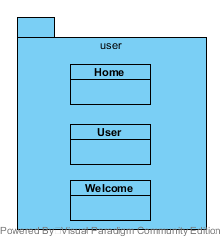
\includegraphics[scale=4, max width=\textwidth, max height=\myheight]{../img/diagrammiClassi/client/controller/user.png}
		\caption{Diagramma package - client::controller::user}
	\end{figure}
\end{center}\hypertarget{client::controller::user::Welcome}{}
\subsubsubsection[Welcome]{client::controller::user::Welcome}
\begin{figure}[H]
	\centering
	\begin{tikzpicture}
	\umlclass{client::controller::user::Welcome} {--answerService : AnswerService\\--rootScope : \$rootScope\\--scope : \$scope}{+Welcome()}
	\end{tikzpicture}
	\caption{Diagramma classe - client::controller::user::Welcome}
\end{figure}\begin{description}
\item[Descrizione] \hfill \\
Classe che si occupa della visualizzazione della pagina di benvenuto
\item[Relazioni con altre classi] \hfill \\
\vspace{-7mm}
\begin{description}
	\item[\hyperlink{client::model::service::AnswerService}{client::model::service::AnswerService}] \hfill \\
	Relazione uscente, campo dati che rappresenta un oggetto AnswerService
\end{description}

\item[Attributi] \hfill \\
\vspace{-7mm}
\begin{itemize}
	\item answerService : AnswerService $\rightarrow$ campo dati che rappresenta un oggetto AnswerService
	\item rootScope : \$rootScope $\rightarrow$ oggetto di angular che identifica l’elemento con attributo ng-app	
	\item scope : \$scope $\rightarrow$ oggetto di angular che fa riferimento ad una porzione di model di pertinenza di uno specifico controller
\end{itemize}

\item[Metodi] \hfill \\
\vspace{-7mm}
\begin{itemize}
	\item Welcome() $\rightarrow$ costruttore della classe
\end{itemize}

\end{description}

\vspace{0.5cm}
\hypertarget{client::controller::user::Home}{}
\subsubsubsection[Home]{client::controller::user::Home}
\begin{figure}[H]
	\centering
	\begin{tikzpicture}
	\umlclass{client::controller::user::Home} {--cookies : \$cookies\\--location : \$location\\--rootScope : \$rootScope\\--sessionService : SessionService\\--scope : \$scope}{+logout() : void\\+Logout(scope : Object, rootScope : Object, sessionService : SessionService, cookies : Object)}
	\end{tikzpicture}
	\caption{Diagramma classe - client::controller::user::Home}
\end{figure}\begin{description}
\item[Descrizione] \hfill \\
Classe che si occupa della gestione della home page di un utente generico registrato
\item[Relazioni con altre classi] \hfill \\
\vspace{-7mm}
\begin{description}
	\item[\hyperlink{client::model::service::SessionService}{client::model::service::SessionService}] \hfill \\
	Relazione uscente, campo dati che rappresenta un oggetto SessionService
\end{description}

\item[Attributi] \hfill \\
\vspace{-7mm}
\begin{itemize}
	\item cookies : \$cookies $\rightarrow$ oggetto di angular che permette di manipolare i cookies
	\item location : \$location $\rightarrow$ oggetto di angular che analizza l'URL nella barra degli indirizzi del browser e lo rende disponibile all'applicazione
	\item rootScope : \$rootScope $\rightarrow$ oggetto di angular che identifica l’elemento con attributo ng-app
	\item sessionService : SessionService $\rightarrow$ campo dati che rappresenta un oggetto SessionService
	\item scope : \$scope $\rightarrow$ oggetto di angular che fa riferimento ad una porzione di model di pertinenza di uno specifico controller
\end{itemize}

\item[Metodi] \hfill \\
\vspace{-7mm}
\begin{itemize}
	\item logout() : void $\rightarrow$ esegue il logout dell'utente che è autenticato distruggendo i cookies di sessione
	\item Logout(scope : Object, rootScope : Object, sessionService : SessionService, cookies : Object) $\rightarrow$ costruttore della classe\begin{itemize}
		\item scope $\rightarrow$ oggetto di angular che fa riferimento ad una porzione di model di pertinenza di uno specifico controller
		\item rootScope $\rightarrow$ oggetto di angular che identifica l’elemento con attributo ng-app
		\item sessionService $\rightarrow$ campo dati che rappresenta un oggetto SessionService
		\item cookies $\rightarrow$ oggetto di angular che permette di manipolare i cookies
	\end{itemize}
	
\end{itemize}

\end{description}

\vspace{0.5cm}
\hypertarget{client::controller::user::User}{}
\subsubsubsection[User]{client::controller::user::User}
\begin{figure}[H]
	\centering
	\begin{tikzpicture}
	\umlclass{client::controller::user::User} {--scope : \$scope\\--check : Check\\--rootScope : \$rootScope\\--userService : UserService\\--errorPassword : Error\\--errorInformation : Error\\--userName : String\\--newPassword : String\\--fullName : String\\--repeatPassword : String\\--oldPassword : String\\--successInformation : boolean\\--successPassword : boolean}{+User(check : Check, rootScope : Object, scope : Object, userService : UserService)\\+checkFullName() : boolean\\+checkPassword() : boolean\\+checkUserName() : boolean\\+checkRepeatPassword() : boolean\\+submitInformation() : void\\+submitPassword() : void\\+getErrorPassword() : Error\\+getErrorInformation() : Error\\+getUserName() : String\\+getNewPassword() : String\\+getFullName() : String\\+getRepeatPassword() : String\\+getOldPassword() : String\\+getSuccessInformation() : boolean\\+getSuccessPassword() : boolean\\+setErrorPassword(errorPassword : Error) : void\\+setErrorInformation(errorInformation : Error) : void\\+setUserName(userName : String) : void\\+setNewPassword(newPassword : String) : void\\+setFullName(fullName : String) : void\\+setRepeatPassword(repeatPassword : String) : void\\+setOldPassword(oldPassword : String) : void\\+setSuccessInformation(successInformation : boolean) : void\\+setSuccessPassword(successPassword : boolean) : void}
	\end{tikzpicture}
	\caption{Diagramma classe - client::controller::user::User}
\end{figure}\begin{description}
\item[Descrizione] \hfill \\
Classe per la gestione del profilo di un'utente generico registrato
\item[Relazioni con altre classi] \hfill \\
\vspace{-7mm}
\begin{description}
	\item[\hyperlink{client::util::Check}{client::util::Check}] \hfill \\
	Relazione uscente, campo dati che rappresenta un oggetto Check
	\item[\hyperlink{client::model::service::UserService}{client::model::service::UserService}] \hfill \\
	Relazione uscente, campo dati che rappresenta un oggetto UserService
	\item[\hyperlink{client::model::data::Error}{client::model::data::Error}] \hfill \\
	Relazione uscente, oggetto che rappresenta un errore da visualizzare all'utente sulla password
	\item[\hyperlink{client::model::data::Error}{client::model::data::Error}] \hfill \\
	Relazione uscente, oggetto che rappresenta un errore da visualizzare all'utente sui dati inseriti
\end{description}

\item[Attributi] \hfill \\
\vspace{-7mm}
\begin{itemize}
	\item scope : \$scope $\rightarrow$ oggetto di angular che fa riferimento ad una porzione di model di pertinenza di uno specifico controller
	\item check : Check $\rightarrow$ campo dati che rappresenta un oggetto Check
	\item rootScope : \$rootScope $\rightarrow$ oggetto di angular che identifica l’elemento con attributo ng-app
	\item userService : UserService $\rightarrow$ campo dati che rappresenta un oggetto UserService
	\item errorPassword : Error $\rightarrow$ oggetto che rappresenta un errore da visualizzare all'utente sulla password
	\item errorInformation : Error $\rightarrow$ oggetto che rappresenta un errore da visualizzare all'utente sui dati inseriti
	\item userName : String $\rightarrow$ rappresenta il campo userName nella View
	\item newPassword : String $\rightarrow$ rappresenta il campo newPassword nella View	
	\item fullName : String $\rightarrow$ rappresenta il campo fullName nella View
	\item repeatPassword : String $\rightarrow$ rappresenta il campo repeatPassword nella view	
	\item oldPassword : String $\rightarrow$ rappresenta il campo oldPassword nella view
	\item successInformation : boolean $\rightarrow$ rappresenta se visualizzare il messaggio di invio con successo dei dati utente
	\item successPassword : boolean $\rightarrow$ rappresenta se visualizzare il messaggio di invio con successo dei dati password utente
\end{itemize}

\item[Metodi] \hfill \\
\vspace{-7mm}
\begin{itemize}
	\item User(check : Check, rootScope : Object, scope : Object, userService : UserService) $\rightarrow$ costruttore della classe\begin{itemize}
		\item check $\rightarrow$ campo dati che rappresenta un oggetto Check
		\item rootScope $\rightarrow$ oggetto di angular che identifica l’elemento con attributo ng-app
		\item scope $\rightarrow$ oggetto di angular che fa riferimento ad una porzione di model di pertinenza di uno specifico controller
		\item userService $\rightarrow$ campo dati che rappresenta un oggetto UserService
	\end{itemize}
	
	\item checkFullName() : boolean $\rightarrow$ controlla se il nome inserito ha i requisiti minimi richiamando il relativo metodo nella classe Check
	\item checkPassword() : boolean $\rightarrow$ controlla se la password inserita ha i requisiti minimi richiamando il relativo metodo nella classe Check
	\item checkUserName() : boolean $\rightarrow$ controlla se lo username abbia i requisiti minimi richiamando il relativo metodo nella classe Check
	\item checkRepeatPassword() : boolean $\rightarrow$ controlla se la password sia uguale a quella inserita nel campo "Ripeti password"
	\item submitInformation() : void $\rightarrow$ invia i dati dell'utente al servizio che ne effettua l'aggiornamento
	\item submitPassword() : void $\rightarrow$ invia i dati sulla password dell'utente modificata al servizio che ne effettua l'aggiornamento
	\item getErrorPassword() : Error $\rightarrow$ metodo che restituisce il valore del campo dati errorPassword
	\item getErrorInformation() : Error $\rightarrow$ metodo che restituisce il valore del campo dati errorInformation
	\item getUserName() : String $\rightarrow$ metodo che restituisce il valore del campo dati userName
	\item getNewPassword() : String $\rightarrow$ metodo che restituisce il valore del campo dati newPassword
	\item getFullName() : String $\rightarrow$ metodo che restituisce il valore del campo dati fullName
	\item getRepeatPassword() : String $\rightarrow$ metodo che restituisce il valore del campo dati repeatPassword
	\item getOldPassword() : String $\rightarrow$ metodo che restituisce il valore del campo dati oldPassword
	\item getSuccessInformation() : boolean $\rightarrow$ metodo che restituisce il valore del campo dati successInformation
	\item getSuccessPassword() : boolean $\rightarrow$ metodo che restituisce il valore del campo dati successPassword
	\item setErrorPassword(errorPassword : Error) : void $\rightarrow$ metodo che cambia il valore del campo dati errorPassword\begin{itemize}
		\item errorPassword $\rightarrow$ oggetto che rappresenta un errore da visualizzare all'utente sulla password
	\end{itemize}
	
	\item setErrorInformation(errorInformation : Error) : void $\rightarrow$ metodo che cambia il valore del campo dati errorInformation\begin{itemize}
		\item errorInformation $\rightarrow$ oggetto che rappresenta un errore da visualizzare all'utente sui dati inseriti
	\end{itemize}
	
	\item setUserName(userName : String) : void $\rightarrow$ metodo che cambia il valore del campo dati userName\begin{itemize}
		\item userName $\rightarrow$ rappresenta il campo userName nella View
	\end{itemize}
	
	\item setNewPassword(newPassword : String) : void $\rightarrow$ metodo che cambia il valore del campo dati newPassword\begin{itemize}
		\item newPassword $\rightarrow$ rappresenta il campo newPassword nella View	
	\end{itemize}
	
	\item setFullName(fullName : String) : void $\rightarrow$ metodo che cambia il valore del campo dati fullName\begin{itemize}
		\item fullName $\rightarrow$ rappresenta il campo fullName nella View
	\end{itemize}
	
	\item setRepeatPassword(repeatPassword : String) : void $\rightarrow$ metodo che cambia il valore del campo dati repeatPassword\begin{itemize}
		\item repeatPassword $\rightarrow$ rappresenta il campo repeatPassword nella view	
	\end{itemize}
	
	\item setOldPassword(oldPassword : String) : void $\rightarrow$ metodo che cambia il valore del campo dati oldPassword\begin{itemize}
		\item oldPassword $\rightarrow$ rappresenta il campo oldPassword nella view
	\end{itemize}
	
	\item setSuccessInformation(successInformation : boolean) : void $\rightarrow$ metodo che cambia il valore del campo dati successInformation\begin{itemize}
		\item successInformation $\rightarrow$ rappresenta se visualizzare il messaggio di invio con successo dei dati utente
	\end{itemize}
	
	\item setSuccessPassword(successPassword : boolean) : void $\rightarrow$ metodo che cambia il valore del campo dati successPassword\begin{itemize}
		\item successPassword $\rightarrow$ rappresenta se visualizzare il messaggio di invio con successo dei dati password utente
	\end{itemize}
	
\end{itemize}

\end{description}

\vspace{0.5cm}
\subsection{client::util}
Il package che contiene le classi di utilità del client.\begin{center}
	\begin{figure}[H]
		\centering 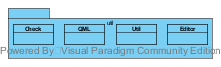
\includegraphics[scale=4, max width=\textwidth, max height=\myheight]{../img/diagrammiClassi/client/util.png}
		\caption{Diagramma package - client::util}
	\end{figure}
\end{center}\hypertarget{client::util::Check}{}
\subsubsection[Check]{client::util::Check}
\begin{figure}[H]
	\centering
	\begin{tikzpicture}
	\umlclass{client::util::Check} {}{+checkPassword(password : String) : boolean\\+checkUserName(userName : String) : boolean\\+checkTitle(title : String) : boolean\\+Check()}
	\end{tikzpicture}
	\caption{Diagramma classe - client::util::Check}
\end{figure}\begin{description}
\item[Descrizione] \hfill \\
Classe che controlla se la password,  l'userName o titolo rispettino il formato scelto
\item[Relazioni con altre classi] \hfill \\
\vspace{-7mm}
\begin{description}
	\item[\hyperlink{client::controller::public::LogIn}{client::controller::public::LogIn}] \hfill \\
	Relazione entrante, campo dati che rappresenta un oggetto Check
	\item[\hyperlink{client::controller::public::SignUp}{client::controller::public::SignUp}] \hfill \\
	Relazione entrante, campo dati che rappresenta un oggetto Check
	\item[\hyperlink{client::controller::user::User}{client::controller::user::User}] \hfill \\
	Relazione entrante, campo dati che rappresenta un oggetto Check
\end{description}

\item[Metodi] \hfill \\
\vspace{-7mm}
\begin{itemize}
	\item checkPassword(password : String) : boolean $\rightarrow$ metodo che controlla la conformità della password rispetto ai parametri scelti: che sia maggiore o uguale a 6 caratteri\begin{itemize}
		\item password $\rightarrow$ contiene la password da controllare  
	\end{itemize}
	
	\item checkUserName(userName : String) : boolean $\rightarrow$ metodo che controlla la conformità dell'username rispetto ai parametri scelti: che sia maggiore o uguale a 6 caratteri\begin{itemize}
		\item userName $\rightarrow$ contiene il username da controllare 
	\end{itemize}
	
	\item checkTitle(title : String) : boolean $\rightarrow$ metodo che controlla la conformità del titolo rispetto ai parametri scelti: che non sia vuoto\begin{itemize}
		\item title $\rightarrow$ contiene il titolo da controllare 
	\end{itemize}
	
	\item Check() $\rightarrow$ costruttore della classe
\end{itemize}

\end{description}

\vspace{0.5cm}
\hypertarget{client::util::Util}{}
\subsubsection[Util]{client::util::Util}
\begin{figure}[H]
	\centering
	\begin{tikzpicture}
	\umlclass{client::util::Util} {}{+alert(message : String) : void\\+confirm(message : String) : boolean\\+Util()}
	\end{tikzpicture}
	\caption{Diagramma classe - client::util::Util}
\end{figure}\begin{description}
\item[Descrizione] \hfill \\
Classe che espone metodi pubblici utili a varie classi del sistema
\item[Relazioni con altre classi] \hfill \\
\vspace{-7mm}
\begin{description}
	\item[\hyperlink{client::controller::teacher::ManageQuestions}{client::controller::teacher::ManageQuestions}] \hfill \\
	Relazione entrante, campo dati che rappresenta un oggetto Util
	\item[\hyperlink{client::controller::teacher::ManageQuestionnaires}{client::controller::teacher::ManageQuestionnaires}] \hfill \\
	Relazione entrante, campo dati che rappresenta un oggetto Util
	\item[\hyperlink{client::controller::teacher::ManageTags}{client::controller::teacher::ManageTags}] \hfill \\
	Relazione entrante, campo dati che rappresenta un oggetto Util
	\item[\hyperlink{client::controller::student::ExecuteQuestionnaire}{client::controller::student::ExecuteQuestionnaire}] \hfill \\
	Relazione entrante, campo dati che rappresenta un oggetto Util
\end{description}

\item[Metodi] \hfill \\
\vspace{-7mm}
\begin{itemize}
	\item alert(message : String) : void $\rightarrow$ stampa un pop-up con un messaggio\begin{itemize}
		\item message $\rightarrow$ 
	\end{itemize}
	
	\item confirm(message : String) : boolean $\rightarrow$ stampa un messaggio chiedendo all'utente di confermare un'azione\begin{itemize}
		\item message $\rightarrow$ 
	\end{itemize}
	
	\item Util() $\rightarrow$ costruttore della classe
\end{itemize}

\end{description}

\vspace{0.5cm}
\hypertarget{client::util::QML}{}
\subsubsection[QML]{client::util::QML}
\begin{figure}[H]
	\centering
	\begin{tikzpicture}
	\umlclass{client::util::QML} {}{+parse(plainText : String) : Json\\+QML()}
	\end{tikzpicture}
	\caption{Diagramma classe - client::util::QML}
\end{figure}\begin{description}
\item[Descrizione] \hfill \\
Classe che provvede metodi per gestire il QML
\item[Relazioni con altre classi] \hfill \\
\vspace{-7mm}
\begin{description}
	\item[\hyperlink{client::controller::teacher::ManageQuestionnaires}{client::controller::teacher::ManageQuestionnaires}] \hfill \\
	Relazione entrante, campo dati che rappresenta un oggetto QML
	\item[\hyperlink{client::controller::teacher::ManageQuestions}{client::controller::teacher::ManageQuestions}] \hfill \\
	Relazione entrante, campo dati che rappresenta un oggetto QML
	\item[\hyperlink{client::controller::teacher::ManipulateQuestion}{client::controller::teacher::ManipulateQuestion}] \hfill \\
	Relazione entrante, campo dati che rappresenta un oggetto QML
	\item[\hyperlink{client::controller::teacher::ManipulateQuestionnaire}{client::controller::teacher::ManipulateQuestionnaire}] \hfill \\
	Relazione entrante, campo dati che rappresenta un oggetto QML
\end{description}

\item[Metodi] \hfill \\
\vspace{-7mm}
\begin{itemize}
	\item parse(plainText : String) : Json $\rightarrow$ provvede a fare il parsing del QML e restituisce un oggetto Json con i seguenti campi: status è un booleano che rappresenta la validità del QML, type è una stringa che rappresenta il tipo di domanda, body è una stringa che contiene il codice HTML per renderizzare la domanda, answers è un array di possibili risposte, answer rappresenta la risposta esatta.\begin{itemize}
		\item plainText $\rightarrow$ 
	\end{itemize}
	
	\item QML() $\rightarrow$ costruttore della classe
\end{itemize}

\end{description}

\vspace{0.5cm}
\hypertarget{client::util::Editor}{}
\subsubsection[Editor]{client::util::Editor}
\begin{figure}[H]
	\centering
	\begin{tikzpicture}
	\umlclass{client::util::Editor} {}{+editor() : SimpleMDE\\+Editor()}
	\end{tikzpicture}
	\caption{Diagramma classe - client::util::Editor}
\end{figure}\begin{description}
\item[Descrizione] \hfill \\
Classe che si occupa di gestire l'editor per il QML
\item[Relazioni con altre classi] \hfill \\
\vspace{-7mm}
\begin{description}
	\item[\hyperlink{client::controller::teacher::ManipulateQuestion}{client::controller::teacher::ManipulateQuestion}] \hfill \\
	Relazione entrante, campo dati che rappresenta un oggetto Editor
\end{description}

\item[Metodi] \hfill \\
\vspace{-7mm}
\begin{itemize}
	\item editor() : SimpleMDE $\rightarrow$ provvede a creare un editor per il QML
	\item Editor() $\rightarrow$ costruttore della classe
\end{itemize}

\end{description}

\vspace{0.5cm}
\subsection{client::app}
Questo Package ha il compito di fornire la configurazione e avviare il client.\begin{center}
	\begin{figure}[H]
		\centering 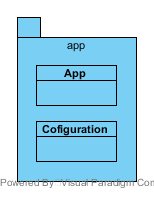
\includegraphics[scale=4, max width=\textwidth, max height=\myheight]{../img/diagrammiClassi/client/app.png}
		\caption{Diagramma package - client::app}
	\end{figure}
\end{center}\hypertarget{client::app::App}{}
\subsubsection[App]{client::app::App}
\begin{figure}[H]
	\centering
	\begin{tikzpicture}
	\umlclass{client::app::App} {}{+App()}
	\end{tikzpicture}
	\caption{Diagramma classe - client::app::App}
\end{figure}\begin{description}
\item[Descrizione] \hfill \\
Classe che si occupa di avviare il client e attivare i moduli angularjs
\item[Metodi] \hfill \\
\vspace{-7mm}
\begin{itemize}
	\item App() $\rightarrow$ costruttore della classe
\end{itemize}

\end{description}

\vspace{0.5cm}
\hypertarget{client::app::Configuration}{}
\subsubsection[Configuration]{client::app::Configuration}
\begin{figure}[H]
	\centering
	\begin{tikzpicture}
	\umlclass{client::app::Configuration} {--remote : String}{+Configuration(remote : String)}
	\end{tikzpicture}
	\caption{Diagramma classe - client::app::Configuration}
\end{figure}\begin{description}
\item[Descrizione] \hfill \\
Classe che rappresenta i parametri di configurazione del client
\item[Relazioni con altre classi] \hfill \\
\vspace{-7mm}
\begin{description}
	\item[\hyperlink{client::model::service::SessionService}{client::model::service::SessionService}] \hfill \\
	Relazione entrante, campo dati che rappresenta un oggetto Configuration
	\item[\hyperlink{client::model::service::UserService}{client::model::service::UserService}] \hfill \\
	Relazione entrante, campo dati che rappresenta un oggetto Configuration
	\item[\hyperlink{client::model::service::TagService}{client::model::service::TagService}] \hfill \\
	Relazione entrante, campo dati che rappresenta un oggetto Configuration
	\item[\hyperlink{client::model::service::QuestionnaireService}{client::model::service::QuestionnaireService}] \hfill \\
	Relazione entrante, campo dati che rappresenta un oggetto Configuration
	\item[\hyperlink{client::model::service::QuestionService}{client::model::service::QuestionService}] \hfill \\
	Relazione entrante, campo dati che rappresenta un oggetto Configuration
	\item[\hyperlink{client::model::service::RoleService}{client::model::service::RoleService}] \hfill \\
	Relazione entrante, campo dati che rappresenta un oggetto Configuration
	\item[\hyperlink{client::model::service::AnswerService}{client::model::service::AnswerService}] \hfill \\
	Relazione entrante, campo dati che rappresenta un oggetto Configuration
\end{description}

\item[Attributi] \hfill \\
\vspace{-7mm}
\begin{itemize}
	\item remote : String $\rightarrow$ rappresenta l'indirizzo verso cui il client effettua le richieste REST
\end{itemize}

\item[Metodi] \hfill \\
\vspace{-7mm}
\begin{itemize}
	\item Configuration(remote : String) $\rightarrow$ costruttore della classe\begin{itemize}
		\item remote $\rightarrow$ rappresenta l'indirizzo verso cui il client effettua le richieste REST
	\end{itemize}
	
\end{itemize}

\end{description}